\documentclass[12pt]{article}

% TEMPLATE DEFAULT PACKAGES
\usepackage{amssymb,amsmath,amsfonts,eurosym,geometry,ulem,graphicx,caption,color,setspace,sectsty,comment,footmisc,caption,natbib,pdflscape,subfigure,array,hyperref,adjustbox}

% ADDED PACKAGES FOR THIS MANUSCRIPT
\usepackage{mathptmx,multirow,titlesec,threeparttable,tabu,booktabs,titlesec,threeparttable,mathtools,bm,bbm}
% endfloat,

% SECTION TITLE SETTINGS
\titlelabel{\thetitle.\enskip}
\titleformat*{\section}{\large\bfseries}
\titleformat*{\subsection}{\normalsize\bfseries}

% COLUMN TYPES
\newcolumntype{L}[1]{>{\raggedright\let\newline\\\arraybackslash\hspace{0pt}}m{#1}}
\newcolumntype{C}[1]{>{\centering\let\newline\\\arraybackslash\hspace{0pt}}m{#1}}
\newcolumntype{R}[1]{>{\raggedleft\let\newline\\\arraybackslash\hspace{0pt}}m{#1}}

% MARGINS AND SPACING
\normalem
%\onehalfspacing
\geometry{left=1.0in,right=1.0in,top=1.0in,bottom=1.0in}

% SPECIAL CELL 
\newcommand{\specialcell}[2][c]{%
	\begin{tabular}[#1]{@{}l@{}}#2\end{tabular}}

\begin{document}

\begin{titlepage}
\title{Public Housing Spillovers \\ in a Developing Country\thanks{We are grateful to Matthew Turner, Jesse Shapiro, John Friedman, Andrew Foster, Brian Knight, and Daniel Bjorkegren for their feedback, advice and support.  We also thank Adelaide Steedley and the Centre for Affordable Housing and Finance in Africa as well as Geo-Terra Image for generous research guidance and for providing excellent data.  Any opinions and conclusions expressed herein are those of the authors and do not necessarily represent the views of the the Federal Trade Commission or its Commissioners.}}
\vspace{2mm}
\author{Benjamin Bradlow\\[-0.4em] \normalsize{\it Brown University}\\
 \\ 
 Stefano Polloni\thanks{Department of Economics, Brown University, Box B, Providence, RI 02912  E-mail: stefano\textunderscore polloni@brown.edu}\\[-0.4em] \normalsize{\it Brown University}\\ 
 \\
  William Violette \\[-0.4em] \normalsize{\it Federal Trade Commission}\\
 \\ 
  }
\vspace{30mm}
\date{\vspace{5mm}This Version: \today}
\maketitle
\begin{abstract}
 We estimate economic spillovers from a large public housing program in South Africa using geocoded deeds records and census data.  With a differences-in-differences design, we find that public housing projects lead to a 16\% decline in nearby formal house prices as well as large increases in the density of nearby informal housing.  We attribute this decline prices in the formal market to negative congestion externalities caused by informal housing growth.  Our results provide evidence that public housing may interact with nearby informal housing supply producing unintended consequences for local development.
 %\\
%\vspace{0in}\\
%\textbf{Keywords:} traffic externalities; street livability; urban policy; housing market.\\
%\vspace{0in}\\
%\textbf{JEL Codes:} O18; H4; R2; R4.\\
\bigskip
\end{abstract}
\setcounter{page}{0}
\thispagestyle{empty}
\end{titlepage}
\pagebreak \newpage

\doublespacing

\section{Introduction} \label{sec:introduction}

In developing countries, 30\% of urban populations live in slums where households often suffer from high rates of crime, low access to infrastructure, insecure property rights, and unsanitary conditions (\cite{mdg}).  These negative congestion externalities often combine to create poverty traps, preventing long-term economic development (\cite{10.1257/jep.27.4.187}). Governments have responded by replacing slums with new homes and moving slum dwellers to public housing projects.  These policies are intended to provide not only direct health and economic benefits to recipients, but also greater incentives for neighbors to invest in their homes and communities, reducing negative externalities and steering communities away from poverty traps.  At the same time, public housing can also attract nearby slum growth by improving access to bulk services like water and sanitation as well as providing undeveloped land within and nearby housing projects.  In this way, public housing projects may ultimately exacerbate the same negative externalities that they were designed to remediate.

% While these policies aim to reduce slum growth
%While these policies are often motivated by immediate health and economic benefits for recipients, economic theory emphasizes how public housing can provide incentives for neighbors to invest more in their own homes and communities, reducing negative externalities and steering communities away from poverty traps.
% In this paper, we document another
% We find that these policies can have 

In this paper, we analyze the impacts of public housing on the development of surrounding neighborhoods.  We study a large-scale housing program in South Africa, which has allocated over 4.3 million dwellings and houses over 13\% of the total population (\cite{dhsreports}; GHS [2009-2013]).  Already one of the largest housing programs in the developing world, this program continues to respond to large backlogs in housing demand with an even mix of upgrading slum areas with new houses as well as constructing stand-alone developments.  This program is intended to not only serve as ``a key strategy for poverty alleviation'' for direct beneficiaries, but also generate community-wide benefits, ``leveraging growth in the economy,'' ``combating crime, promoting social cohesion and improving quality of life for the poor,'' and ``utilizing housing as an instrument for the development of sustainable human settlements, in support of spatial restructuring'' (\cite{bng}). 

We combine administrative records for over 50 completed housing projects with data on property transactions, demographics, and building construction to measure the local impacts of these projects.  We estimate a 16\% decline in formal residential home prices within 400 meters of a project that persists three years after construction.  We find evidence of greater access to services and improved home quality within project areas while surrounding neighborhoods experience substantial growth in informal housing.  To interpret these findings, we develop a simple model of residential choice with congestion externalities.  We model public housing as a subsidy for construction costs in both the immediate formal housing market as well as surrounding informal housing markets.  These subsidies cause growth in nearby informal housing, which exacerbates congestion externalities and generate declines in formal home prices.

% the welfare effects..
% attribute the local decline in housing prices in the formal market to greater externalities imposed 
% To understand the welfare implications of this policy, we also develop a model similar to... 
%We then use heterogeneity in the extent to which projects eradicate existing slums as a natural experiment to quantify negative externalities from slum areas.  Our estimates imply that increasing slum density by [XX]\% leads to a [XX]\% decline in local housing prices.  We find some evidence that this effect scales non-linearly with the size of the housing projects, which has theoretical implications for the extent to which slum areas represent poverty traps.

To identify these effects, we use a differences-in-differences strategy leveraging both the exact timing of housing project construction as well as the precise geographic proximity of surrounding areas.  Like prior studies in the US, the substantial uncertainty in project timing due to difficulties coordinating many stakeholders and sources of funding limits the extent to which local housing markets are able to anticipate these projects (\cite{diamond2016wants}; \cite{serihistory}).  To address the potential endogenous placement of housing projects, we use planned but unconstructed projects as counterfactuals and detect no impacts of these projects on local housing markets.

Our negative spillover estimates stand in contrast to a large literature in development that has found positive impacts of public housing on direct recipients.  Relying on small-scale experimental designs, previous studies have linked public housing to improvements in employment outcomes (\cite{franklin2016enabled}), self-reported wellbeing (\cite{galiani2017shelter}; \cite{devoto2012happiness}), and child health outcomes (\cite{cattaneo2009housing}).  Data limitations both in finding a large enough sample of housing projects and in identifying outcomes at a precise spatial scale have prevented previous studies from identifying spillover effects.  Taken alongside these previous studies, our findings suggest that policymakers may want to consider weighing direct benefits to recipients against potential negative effects to the local housing neighborhoods in designing future housing policy.

We proceed by first providing background on the South African housing program in Section~\ref{section:background}.  In Section~\ref{section:model}, we develop a model of residential choice and housing externalities to help to interpret the results. Section~\ref{section:data} describes the data used to measure outcomes and details our approach to identifying housing projects while Section~\ref{section:descriptives} provides descriptive evidence.  We present spillover results for residential home prices in Section~\ref{section:resultsprices} and demographic outcomes in Section~\ref{section:resultscensus}.  Section~\ref{section:discussion} includes a discussion of our findings before Section~\ref{section:conclusion} provides some concluding thoughts.


\section{Background: Where are houses built?}\label{section:background}

Between 2000 and 2010, subsidized housing efforts in South Africa have primarily focused on constructing and allocating single-story, two-room (30 to 40 square meter) dwellings to households in groups of 50 to 500 per project.  These housing projects are evenly divided between two categories (\cite{dhsreports}):
\begin{enumerate}
	\item  \textbf{Greenfield developments} involve the construction of housing projects primarily on undeveloped state-owned land although in some cases, municipalities will work with private developers to purchase inexpensive, undeveloped private land for these projects.  Finding undeveloped land often requires policymakers to locate these projects far from city centers and economic opportunities.  
	\item  \textbf{In-situ upgradings} replace existing informal settlements with housing developments.\footnote{While in some cases these programs refer simply to the provision of land titles and municipal services (water, electricity, etc.), this paper focuses on cases where informal settlements are replaced by fully-serviced, single-story houses.}  Since informal settlements are often located closer to city centers, the resulting housing projects may provide better employment opportunities (\cite{serihistory}).
\end{enumerate}
Facing substantial housing demand, the Department of Human Settlements has continued to issue grants to provincial governments to keep the rate of yearly housing allocations roughly constant (\cite{dhsreports}).  While the location and types of projects are determined by provincial and municipal governments, construction is subcontracted to private developers who also act as project managers assisting in the allocation of houses to beneficiaries (\cite{seriq}).

Since housing projects require coordination between many stakeholders, these projects often face unanticipated delays and cancellations due to labor and land procurement issues, difficulties gaining support from local government agencies, environmental impact assessments, and inadequate bulk infrastructure provision (\cite{dhsreports}).  In one example, political disagreements with local stakeholders led to the abandonment of a large project near Johannesburg (\cite{protest}).

\subsection{Background: Who are the beneficiaries?}

The National Department of Human Settlements issues guidelines for eligibility and maintains an official waiting list for eligible households for greenfield developments.  Eligibility requires citizenship, no previous property ownership, being married or having financial dependents, and having a monthly household income below R3,500 (\cite{seriq}).\footnote{The Gauteng Province has implemented their own waiting list since 2008 in order to exert greater control over the allocation process.}  The share of households reporting at least one member on the waiting list has remained stable at over 13\% from 2009 to 2013.\footnote{This figure is calculated from the General Household Surveys from 2009 to 2013}  Before construction, each project is assigned beneficiaries in a first-come, first-served basis according to the waiting list in their province or municipality.  For in-situ upgrading projects, previous inhabitants of informal settlements receive renovated houses while any remaining houses are allocated according to the housing waiting list.

In practice, these guidelines are only loosely followed.  Recent reports point to cases of corruption in the allocation of houses while in some instances, housing projects are organized with the assistance of local community groups who ultimately select the beneficiaries (\cite{seriq}; \cite{casestudytinazonke}).  Research suggests that beneficiaries are often selected over the course of project construction and sometimes even after construction has finished (\cite{seriq}).

Beneficiaries are expected to pay a small one-time payment in order to receive title for their houses.  Guidelines also prevent beneficiaries from reselling their houses within their first 7 years of ownership.  Despite these guidelines, only 82\% of project houses are reported being still occupied by their original beneficiaries within five years of construction.\footnote{This figure is calculated from the General Household Surveys from 2009 to 2013}  Anecdotal evidence suggests that project managers are aware of active secondary markets but have difficulty policing these transactions (\cite{resale}).



\section{A Model of Residential Choice and Public Housing}\label{section:model}

We develop a simple model of residential choice in order to both guide the reduced form empirical analysis as well as provide a framework evaluating the welfare effects of public housing policy.  The key insight of the model is that while public housing projects provide high-quality houses and infrastructure, they also cross-subsidize informal housing markets, which can exacerbate congestion externalities and decrease prices in the formal market.

\subsection*{Basic Setup}
A city is comprised of $N$ residential neighborhoods indexed $n\in\{1,...,N\}$.  Each neighborhood has a formal and informal housing sector, indexed $s\in\{F,I\}$.  Each neighborhood is distinguished by its local housing supply and later by negative congestion externalities from informal housing.  All jobs are in the central business district and pay a fixed wage rate, and commuting to the CBD is costly.

\subsection*{Housing Demand}

Measure one of freely-mobile agents inelastically demand one unit of housing. An agent $i$ has idiosyncratic tastes for neighborhoods, represented by the vector $\bm{\epsilon}_i \in \mathbb{R}^{2N}$ of neighborhood-sector specific valuations. The distribution of preferences in the population is given by the continuous and well-behaved function $f(\bm{\epsilon})$ such that $\int f(\bm{\epsilon}) d\bm{\epsilon} = 1$.
The indirect utility of individual $i$ living in sector $s$ of neighborhood $n$ is given by:
\begin{equation*}
\begin{aligned}
u_{ins} \,& =\, A_{ns}\,-\, R_{ns} \,+\, \epsilon_{ins} \\
        \,& =\, v_{ns} \,+\, \epsilon_{ins}
\end{aligned}
\end{equation*}
 where $A_{ns}$ may be interpreted as the net-of-commuting and amenity-adjusted wage received in $n$ when living in sector $s$, $R_{ns}$ is the rental rate of housing, and $\epsilon_{ins}$ is individual $i$'s idiosyncratic taste for neighborhood-sector pair $(n,s)$.  In this framework, neighborhood-sector tastes, $\epsilon_{ins}$, are assumed to be uncorrelated across space and sector.  This assumption rules out cases where households may prefer living closer to certain areas or in certain types of housing.

 For notational convenience, we denote the array of quantities $A_{ns}$, $R_{ns}$ and $\epsilon_{ins}$ in their matrix form as $\bm{A}$, $\bm{R}$ and $\bm{\epsilon}_i$. Individual $i$ takes exogenous quantities $\{\bm{A},\bm{\epsilon}_i\}$ and endogenous rents $\bm{R}$ as given, and locates in pair $(n,s)$ yielding the highest indirect utility. Aggregate housing demand $H_{ns}$ in $(n,s)$ is given by:
\begin{equation*}
\begin{aligned}
H_{ns} \,\,& =\,\, \int I\Big( \, u_{ins} \,=\, \max_{n's'}\{u_{in' s'} \,\,|\,\, \bm{A},\bm{R}\,\} \Big)f(\bm{\epsilon}) d\bm{\epsilon}    \\[.2em]
        \,\,& =\,\, D_{ns}(\bm{A},\bm{R})
\end{aligned}
\end{equation*}


\subsection*{Housing Supply}

 Neighborhoods are endowed with $L_n$ units of land. A share $\theta_{nF}$ of the total land stock is available for formal residential development, while the rest, $\theta_{nI} = 1-\theta_{nF}$, is vacant or public land suited for informal housing. We assume that $\theta_{nF}$ is determined exogenously. In each sector, price-taking landlords supply housing by combining land and materials $M$ with CRS technology $q(L,M)$. Materials are supplied at fixed cost $c$ on a large national market. Because land is fixed in every market, the marginal cost of housing is increasing. The government may also choose to subsidize housing in market $(n,s)$ at a rate of $\delta_{ns}$ per unit. The inverse supply curve in $(n,s)$ is:
\begin{equation*}
R_{ns} \,\, =\,\, S(H_{ns},\theta_{ns}L_n) - \delta_{ns}
\end{equation*} \\[-1.99em]
 where $\partial S/\partial H > 0$ and $\partial S/\partial L < 0$. For notational convenience, we denote the array of quantities $H_{nh}$, $L_n$ and $\theta_n$ in their vector form as $\bm{H}$, $\bm{L}$ and $\bm{\theta}$, respectively.

\subsection*{Equilibrium}

Given density $f(\bm{\epsilon})$ and the exogenous quantities $\{\bm{A},\bm{L},\bm{\theta}\}$, an equilibrium in this city consists of rents $\bm{R}^*$ and housing quantities $\bm{H}^*$ such that all housing markets clear, that is, $\forall (n,h)$:
\begin{equation}
\begin{aligned}
& H^*_{ns} \,\, =\,\, D_{ns}(\bm{A}, \bm{R}^*) \\
\text{and}\quad & R^*_{ns} \,\, =\,\, S(H^*_{ns},\theta_{ns}L_n) - \delta_{ns} \text{,}
\end{aligned}
\end{equation}\\[-1.99em]\\[-1.99em]
 and all agents live somewhere:
\begin{equation*}
\sum_{n}\sum_{s} H^*_{ns} = 1 
\end{equation*} \\[-1.99em]

\subsection*{Welfare Implications of Housing Subsidies}

 The sum of individuals' utility is given by:
\begin{equation*}
U \,\, =\,\, \int \max_{n's'}\{u_{in' s'}\,\,|\,\, \bm{A},\bm{R}^*\,\}f(\bm{\epsilon}) d\bm{\epsilon} 
\end{equation*} \\[-1.99em]
 and total landlords' profit is:
\begin{equation*}
\begin{aligned}
\Pi \,\, &=\,\, \sum_{n}\sum_{s} \Bigg(\,\int_0^{H^*_{ns}} [R^*_{ns} - (S(x,\theta_{ns}L_n) - \delta_{ns})]dx \, \Bigg) \\[.6em]
\,\, &=\,\, \sum_{n}\sum_{s} \Bigg(\, R^*_{ns}H^*_{ns} +  \delta_{ns}H^*_{ns} -  \int_0^{H^*_{ns}}S(x,\theta_{ns}L_n)dx  \,\Bigg)
\end{aligned}
\end{equation*} \\[-1.99em]
 Total social welfare in this economy is therefore $W = U + \Pi$. We are interested in the welfare implications of the government subsidizing formal housing in a subset $\mathcal{N}\subset\{1,...,N\}$ of neighborhoods. Let $\delta_{ns}=\delta$ if $n\in\mathcal{N}$ and $s=F$, and $\delta_{ns}=0$ otherwise.  To characterize the marginal social benefit from the subsidy, $\partial W/\partial \delta$,  we first note a result shown in \cite{busso2013assessing}:

\begin{equation*}
\begin{aligned}
\frac{\partial U}{\partial v_{ns}} \,\, & =\,\, \int \frac{\partial }{\partial v_{ns}} \max_{n's'}\{u_{in' s'}\,\,|\,\, \bm{A},\bm{R}\,\}f(\bm{\epsilon}) d\bm{\epsilon} \\[.6em]
\,\, & =\,\, \int I\Big( \, u_{ins} \,=\, \max_{n's'}\{u_{in' s'} \,\,|\,\, \bm{A},\bm{R}\,\} \Big)f(\bm{\epsilon}) d\bm{\epsilon} \\[.6em]
\,\, & =\,\  H_{ns}
\end{aligned}
\end{equation*} \\[-1.99em]

 Using the above, we write the derivative of total utility with respect to subsidy $\delta$ as:

\begin{equation*}
\frac{\partial U}{\partial\delta} \,\,=\,\,  \sum_{n}\sum_{s}\,\, H^*_{ns}\Big(-\frac{\partial R_{ns}^*}{\partial \delta}\Big) 
\end{equation*} \\[-1.99em]

 The derivative of total profits with respect to $\delta$ is:

\begin{equation*}
\frac{\partial \Pi}{\partial\delta} \,\,=\,\, \sum_{n\in\mathcal{N}} H^*_{nF} \,\,+\,\, \sum_{n}\sum_{s}\, \Big[ H^*_{ns}\frac{\partial R^*_{ns}}{\partial \delta} \,\,+\,\, R^*_{ns}\frac{\partial H^*_{ns}}{\partial \delta} \,\,+\,\, \delta_{ns}\frac{\partial H^*_{ns}}{\partial \delta} \,\,-\,\, \frac{\partial H^*_{ns}}{\partial \delta}\big( R^*_{ns} \,\, + \,\, \delta_{ns} \big) \Big]
\end{equation*} \\[-1.99em]

 Summing and simplifying:

\begin{equation}
\frac{\partial W}{\partial\delta} \,\,=\,\, \frac{\partial U}{\partial\delta} \,\,+\,\, \frac{\partial \Pi}{\partial\delta} \,\,=\,\, \sum_{n\in\mathcal{N}} H^*_{nF}
\end{equation} \\[-1.99em]

 The total cost of the subsidy is given by $TC = \sum_n\sum_s H^*_{ns}\delta_{ns}$ and its marginal cost is thus:
\begin{equation*}
 \frac{\partial TC}{\partial \delta} \,\,=\,\, \sum_{n\in\mathcal{N}} \Big( H^*_{nF} \,\,+\,\, \delta\frac{\partial H^*_{nF}}{\partial \delta} \Big)
 \end{equation*} \\[-1.99em]

  The extra term in this expression relative to (2) represents the marginal deadweight loss from an increase in $\delta$. Unsurprisingly, we find that subsidies in an economy with perfect housing markets lead to economic inefficiencies. Furthermore, the magnitude of these inefficiencies depends critically on the population responses in subsidized markets.

 \subsection*{Housing subsidies with Slum Externalities}

 Densely populated slums pose fire hazards, increase health risks and overburden existing public infrastructure, e.g. water and sewage networks. We consider an external utility cost from informal housing of the form:

\begin{equation*}
A_{ns} \,\,=\,\, \bar{A}_{ns} \,\,+\,\, a\Big(\frac{H_{nI}}{L_n}\Big)
\end{equation*} \\[-1.99em]

 where $a'(.)<0$. With this specification, the private decision of locating in $(n,I)$ negatively impacts all residents in $n$ because of congestion effects. The utility response to $\delta$ now depends on how both rents and amenities change in equilibrium:

\begin{equation*}
\frac{\partial U}{\partial\delta} \,\,=\,\,  \sum_{n}\sum_{s} \,\, H^*_{ns}\Big(a'\Big(\frac{H^*_{nI}}{L_n}\Big)\frac{\partial H^*_{nI}}{L_n\partial \delta}\,\,-\,\,\frac{\partial R_{ns}^*}{\partial \delta}\Big) 
\end{equation*} \\[-1.99em]

 Therefore:

\begin{equation*}
\frac{\partial W}{\partial\delta} \,\,=\,\, \sum_{n\in\mathcal{N}} H^*_{nF} \,\,+\,\, \sum_{n} a'\Big(\frac{H^*_{nI}}{L_n}\Big)\,\frac{\partial H^*_{nI}}{\partial \delta}\,\frac{(H^*_{nF}+H^*_{nI})}{L_n}
\end{equation*} \\[-1.99em]

 Combining the equilibrium conditions in (1) and using the implicit function theorem, it is possible to show formally that $\partial H^*_{nI}/\partial \delta < 0 \,\,\forall n$. The extra term in the above expression -- relative to equation (2) -- represents the marginal welfare {\it gain} from reduced slum density. The subsidy $\delta$ makes formal housing in $\mathcal{N}$ more attractive relative to informal housing. Marginal residents moving to $\mathcal{N}$ make remaining residents better-off because of reduced congestion. The marginal deadweight loss (MDWL) of the subsidy is now :

\begin{equation*}
\begin{aligned}
MDWL \,\,&=\,\, \frac{\partial TC}{\partial \delta} - \frac{\partial W}{\partial \delta} \\[.6em]
     \,\,&=\,\, \sum_{n\in\mathcal{N}} \,\delta\frac{\partial H^*_{nF}}{\partial \delta} \,\,-\,\, \sum_{n} \, a'\Big(\frac{H^*_{nI}}{L_n}\Big)\,\frac{\partial H^*_{nI}}{\partial \delta}\,\frac{(H^*_{nF}+H^*_{nI})}{L_n} \\
\end{aligned}
\end{equation*} \\[-1.99em]

 Efficiency considerations in this setting depend on the population responses in subsidized markets, but also on responses in informal markets and on the shape of slum externality $a(\,)$. We note that $\delta=0$ implies $MDWL<0$, that is, some level of subsidy $\delta$ is welfare improving when compared to no subsidy. This is expected since the social benefits exceed the private benefits of moving from informal to formal housing. 

\subsection*{Subsidy Spillovers}

South Africa's housing program involves low density housing projects as well as large improvements to surrounding infrastructure such as electricity, water, and sanitation to service these new houses.  Both have the additional impact of lowering construction costs for informal housing by providing space in and around housing projects to set up new informal dwellings as well as improving access to bulk services.  Since the policy effectively lowers construction costs for informal housing, we model this by assuming subsidies in the formal sector spillover to the informal sector at no additional cost for the government. Formally, we let $\delta_{ns} = \delta$ if $n\in\mathcal{N}$ and $s=F$, $\delta_{ns} = \alpha\delta$ if $n\in\mathcal{N}$ and $s=I$, and $\delta_{ns} = 0$ otherwise, where $\alpha\in\mathbb{R}^+$. 

Construction cost spillovers for the informal sector alter the welfare implications in two ways. First, suppliers of informal housing benefit from an increase in profit due to the indirect subsidies. Second, for $n\in\mathcal{N}$, the sign of informal housing response $\frac{\partial H^*_{nI}}{\partial\delta}$ is now ambiguous and depends on the magnitude of $\alpha$.\footnote{ This can also be shown formally by combining the equilibrium conditions in (1) and using the implicit function theorem. For $n\in\mathcal{N}^C$, $\frac{\partial H^*_{nI}}{\partial\delta}$ remains unambiguously negative.} We use the notation $\frac{\partial H^*_{nI}}{\partial\delta}(\alpha)$ to represent this dependence. When $\alpha$ is large, the indirect subsidies in $(n,I)$ dominate and net-migration is positive, i.e. $\frac{\partial H^*_{nI}}{\partial\delta}>0$, making incumbent residents in $(n,I)$ and $(n,F)$ worse-off. With similar derivations as above, we obtain:

\begin{equation*}
\frac{\partial W}{\partial\delta} \,\,=\,\, \sum_{n\in\mathcal{N}} \big( H^*_{nF} + \alpha H^*_{nI} \big)  \,\,+\,\, \sum_{n} a'\Big(\frac{H^*_{nI}}{L_n}\Big)\,\frac{\partial H^*_{nI}}{\partial \delta}(\alpha)\,\Big(\frac{H^*_{nF}+H^*_{nI}}{L_n} \Big)
\end{equation*} \\[-1.99em]

 and therefore:

\begin{equation*}
MDWL \,\,=\,\, \sum_{n\in\mathcal{N}} \,\delta\frac{\partial H^*_{nF}}{\partial \delta} \,\,-\,\, \sum_{n\in\mathcal{N}} \alpha H^*_{nI}\,\,-\,\, \sum_{n} \, a'\Big(\frac{H^*_{nI}}{L_n}\Big)\,\frac{\partial H^*_{nI}}{\partial \delta}(\alpha)\,\Big(\frac{H^*_{nF}+H^*_{nI}}{L_n} \Big)
\end{equation*} \\[-1.99em]

\subsection*{Empirical Predictions}

First, in terms of direct impacts, this model predicts by assumption that the housing subsidy program increases local formal and informal housing, improves public services, and attracts informal housing growth in nearby areas.  

Second, informal settlement growth nearby public housing projects exacerbates congestion externalities, depressing housing prices in nearby formal and informal housing markets relative to housing markets further away.  

While this model attributes decreases in nearby home prices to congestion externalities, there may exist other mechanisms that would generate a similar decline in home prices and are not explicitly modeled.  One mechanism includes housing externalities for formal housing where changes in the quality of neighbors' houses directly affects the value of neighboring houses.  If subsidy houses have low quality relative to their neighborhoods, then nearby houses may simply have less amenity value than before.  This theory implies that project houses have lower quality than preexisting formal houses, which can be tested in the data.  Another mechanism would be allowing for heterogeneity in tastes for neighboring households.  If subsidy programs target recipients unlike preexisting households (ie. lower income), then neighboring home prices may decline simply because recipients are undesirable neighbors.  We can similarly test for evidence of changing demographics in project neighborhoods to address this alternative theory. 

%Without congestion externalities, the model predicts no differential change in housing prices near and far from housing projects.  
% In the context of this model, we understand congestion externalities to be a feature of 
%%%We test these hypotheses directly by tracking growth in informal and formal structures within and nearby housing projects as well as improvements in local service provision.
% Second, the model predicts that the increase in informal housing will exacerbate congestion externalities, depressing nearby housing rents in both the informal and formal sectors  
%This model highlights key quantities to be estimated in order to assess the incidence and efficiency of formal housing subsidies. Specifically, welfare considerations depend critically on the magnitude of spillovers $\alpha$, the shape of slum externalities $a(\,)$, and the population (housing) responses in both subsidized formal markets, $\frac{\partial H^*_{nF}}{\partial \delta}\,\,\forall n\in\mathcal{N}$,  and informal markets, $\frac{\partial H^*_{nI}}{\partial \delta}\,\,\forall n$. Empirical analysis should therefore focus on obtaining reliable estimates of theses quantities.

\section{Data}\label{section:data}

Understanding the spillover impacts of public housing requires (1) outcome measures at high spatial and geographic resolutions as well as (2) a precise measure of the location, timing, and size of housing projects.  

%\subsection{Measuring Spillover Outcomes}

We locate housing projects using administrative maps compiled by the Gauteng City Regional Authority.  These records include 642planned housing projects as well as notes on their completion status.\footnote{Since this data comes in the form of overlapping shapefiles, we use the intersection of the shapes excluding tiny shapes below 0.50 square kilometers.}  

To measure formal housing market impacts, we use over 500,000 housing transactions from the South African National Deeds Office covering the universe of transactions for suburbs in the bottom 20\% of the housing market between 2003 and 2011 in the Gauteng Province (including the Johannesburg metro area).\footnote{The bottom 20\% suburbs were selected relative to prices in 2003 and followed every year from 2003 to 2011.  These data were provided by the Affordable Land and Housing Data Centre, which tracks affordable housing markets.}  These data include the price, exact location, plot size, buyer name, and seller name for each transaction.  To isolate spillover effects, we focus on transactions occurring within 1.2 kilometers of a housing project bringing the final sample to around 200,000 transactions.  We exclude the top 1\% of prices as well as prices below 2,500 Rand, which are likely composed of measurement error or the exchange of property title between family members.

Since it is unlikely that government deeds records capture informal housing markets, we also include a building census of all structures in the Gauteng Province in 2001 and 2011.  Using a combination of high-resolution satellite imagery and local field teams, these data record the precise location of each structure, identifying structures within over 30 categories including formal and informal residential dwellings.  Out of 3,817,840structures, this building census includes 1,628,073formal structures and 1,560,345informal structures.  These data serve as both outcome measures of informal housing development as well as additional measures of public housing construction.

For demographic and economic outcomes, we have access to the full census of population and housing for 2001 and 2011, which provides information on housing characteristics, population density, as well as income and employemnt measures.   To spatially link these households in both samples to their corresponding housing projects, we conduct the analysis at the census block level, which is the smallest geography available with 28,437total blocks in Gauteng Province and 20,457within 4 kilometers of a housing project.
%as well as the yearly General Household Survey for 2005 through 2014.  

% The General Household Survey includes additional details on participation in housing programs over time for a random sample of around 35,000 households in the Gauteng Province. 

% Both surveys include information about dwelling type, employment, income, and demographics for each household.  The General Household Survey includes additional details on participation in housing programs over time for a random sample of around 35,000 households in the Gauteng Province.

\subsection{Constructed Housing Projects}

%We construct our primary measure of housing projects by matching a set of known characteristics for housing projects for properties transacted in the deeds data.  This procedure results in spatially distinct clusters that form the definition of housing projects for the empirical analysis (\cite{serihistory}).  Due to data limitations, we are not able to differentiate between greenfield and in-situ upgrading projects in the analysis.

%\subsubsection{Seller Identity}
% prob yes and large : 2770 / 127600 = 2\%

We define projects as successfully constructed when we observe at least some recipients receiving deeds to their new government houses.  Deed transfers are assumed to belong to a housing project if the seller name includes a government, municipality, or large developer.  We exclude deeds flagged as large buildings used for commercial purposes ($<$2\% of transactions) as well as purchase prices that are more than R50,000 above the yearly subsidy value ($<$4\% of remaining transactions).  Using this criteria, we are able to identify over 57 constructed housing projects out of 642planned projects.

This approach may introduces measurement error insofar as we are mis-attributing deeds to housing projects.  We use a limited definition of verified seller names to minimize the chances that unconstructed projects are misclassified as constructed projects.  However, this approach increases the possibility that this definition mistakenly excludes constructed projects.

\begin{figure}
\caption{Top-Five Sellers}\label{figure:topfivesellers}
\centering
\begin{tabu}{lc}
\toprule
 Seller Name & Observations \\
\midrule
City Of Johannesburg Metropolitan Municipality & 29,087  \\
City Of Johannesburg & 27,672  \\
City Of Tshwane Metropolitan Municipality & 24,780  \\
Ekurhuleni Metropolitan Municipality & 21,758  \\
Gauteng Provincial Housing Advisory Board & 13,058  \\
{\bf Total Observations }& {\bf 549,704}  \\
\bottomrule
\end{tabu}

\end{figure}

Descriptive evidence supports our project definition.  First, Figure~\ref{figure:topfivesellers} shows that the top five most frequently occurring seller names clearly correspond to government housing programs in the region.  Second, transaction prices for project houses are strongly clustered around subsidy values.  Figure~\ref{figure:transactionhist} provides a histogram of deed prices under R100,000 for transfers that meet our project definition as well as those that do not.  Government agencies often record either zero price or the value of the subsidy in the deeds, producing substantial bunching at these values compared to non-project transactions.  

%We find some prices scattered away from subsidy values consistent with some measurement error in deeds reporting or miscategorization of non-project properties as project properties.  
%contain a large number of simultaneous deeds transfers from  which can be attributed to a government seller,  or housing authority.  
%In practice, we use a combination of frequent transactions 
%To account for large developers or banks being listed as sellers for housing projects, we also include seller names that appear most frequently.  
%We exclude transactions flagged as large buildings used for commercial purposes ($<$2\% of transactions).  
% above 50,000 : 4,369 / 127,600 = 3.4\%
%Non-project transactions also demonstrate some bunching at round numbers, which may add 

\begin{figure}
\caption{Transaction Price Histogram}\label{figure:transactionhist}
\centering
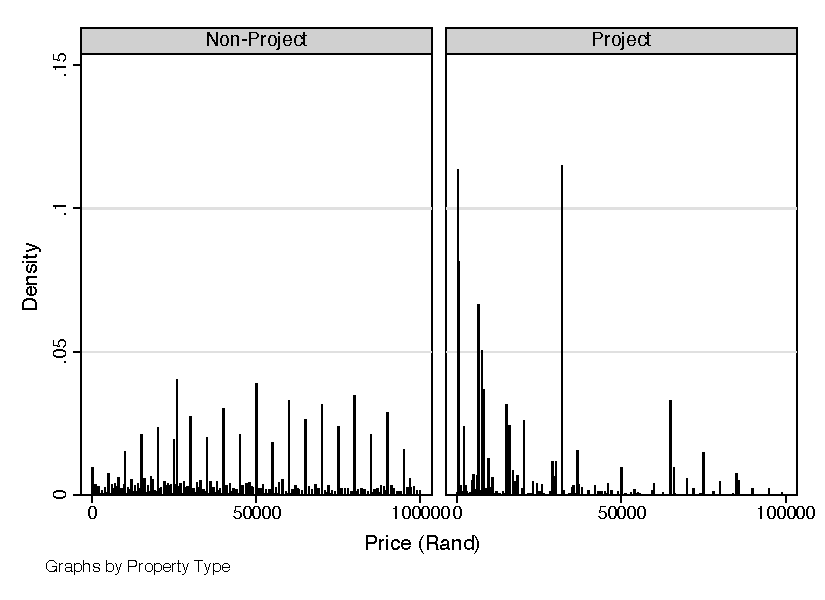
\includegraphics[scale=1]{figures/price_histogram.pdf}\\
Note: Transactions are censored at R100,000.
\end{figure}


We assign a date for each project according to the modal year of deeds.  Figure~\ref{figure:densitytime} indicates the distribution of transaction dates for properties within a 1.2 km buffer around clusters (above panel) and within the selected project areas (below panel).  Project areas exhibit substantial bunching during a single month when projects were completed.  There are also more transactions after the modal year than before the modal year, consistent with either a gradual roll-out for some project areas or immediate resale of projects houses after construction, which would be counter to housing regulations.  

%We then include only clusters where over 50\% of transactions occur during the modal year, which excludes half of total clusters.  This approach helps to exclude incremental projects as well as possible land titling programs, allowing us to leverage the sharp timing of large project construction in our identification.  

Evidence of similar bunching around the modal year for transactions coded as non-project transactions (above panel) would suggest that we may be miscoding project transactions as non-project transactions; instead, we find a smooth pattern relative to the modal year for these non-project transactions.  The slight increase in density around and just following the modal year may also be consistent with housing projects having an immediate impact on local housing markets, which we will explore further below.

\begin{figure}
\caption{Transaction Densities Relative to Modal Project Month}\label{figure:densitytime}
\centering
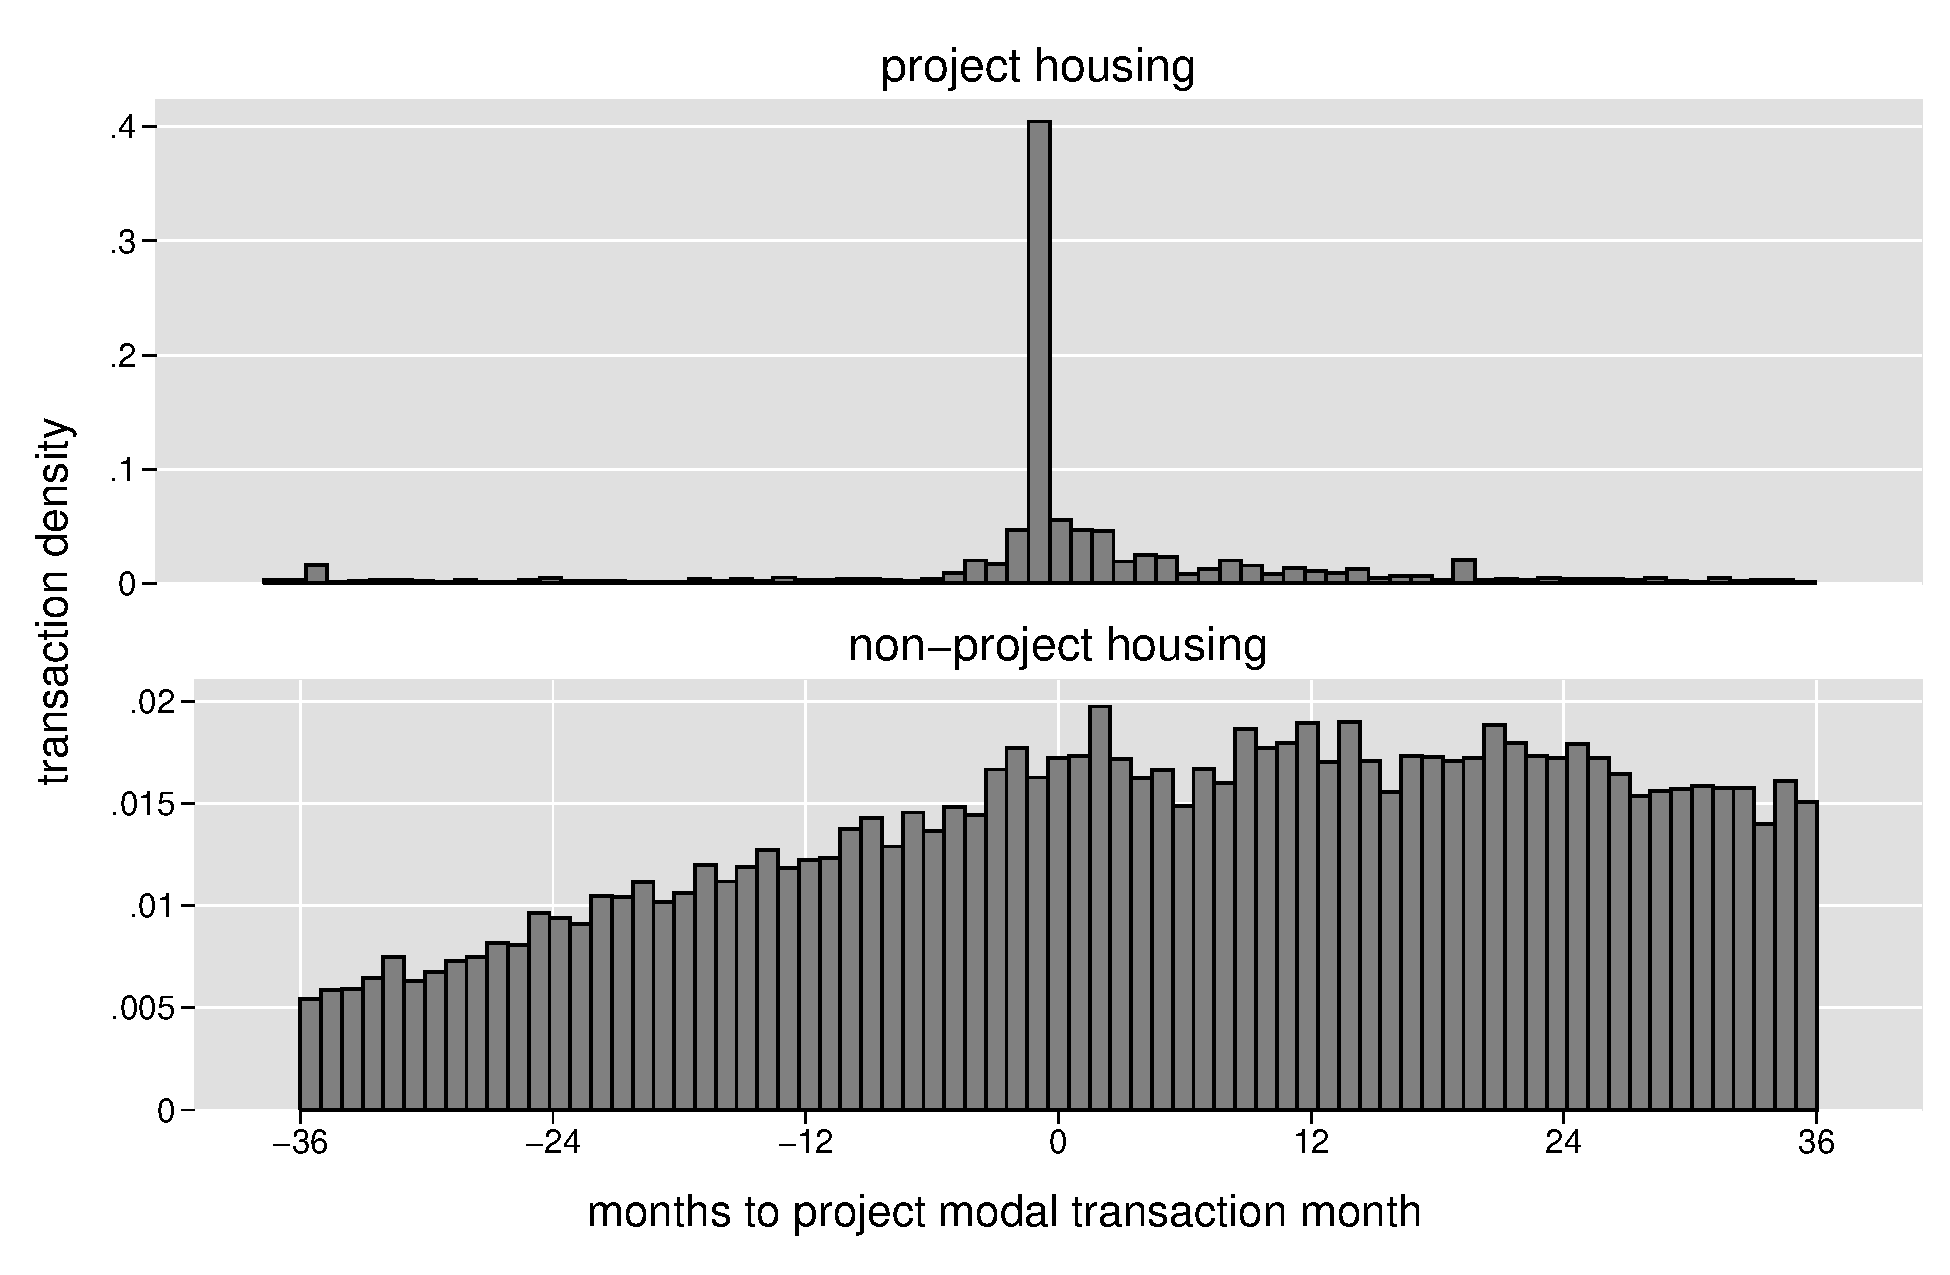
\includegraphics[scale=.5]{figures/summary_densitytime.pdf} \\
The above panel includes transactions within a 1.2 kilometer buffer around a project cluster relative to the modal year of that cluster.  The below panel includes all transactions within the final sample of clusters.
\end{figure}


\subsection{Planned but Unconstructed Housing Projects}



%The administrative spatial data identifies many project areas that do not appear to have received housing projects, as measured by having fewer than 5 housing project transactions per square kilometer.  We use these areas to create a sample of planned but unconstructed housing projects to serve as counterfactuals areas in our analysis.

To construct an estimated completion date for planned but unconstructed housing projects, we digitized National Treasury budget reports that detail the start date, expected completion date, and cost of each housing project.  We use a fuzzy-string matching algorithm with bigrams to successfully link project names from the budget reports for over 300 project names in our administrative spatial data (including both completed and uncompleted projects).  Appendix~\ref{table:stringmatch} compares unmatched and matched projects finding that matched projects have a higher density of formal and informal houses although they are smaller in total area.  We find that for completed projects, the mode transaction year observed in the deeds data falls an average of three years after the start date indicated in the budget reports.  In other words, beneficiaries receive title to their new houses about three years after the housing program is announced in the budget.  Therefore, we assign a expected completion date for unconstructed projects that is three years after the announced start-date in the project.  


\subsection{Assessing Project Measures}

To assess the extent to which our definitions accurately measure housing projects, Figure~\ref{figure:gcrooverlap} maps our cluster definitions on top of administrative data on housing projects.  We see strong overlap between clusters and administrative projects, providing additional support for our deeds-based cluster measure.  A few smaller clusters do not overlap with administrative definitions, which is consistent with the administrative data recording larger, higher-cost projects.  Similarly, administrative boundaries that do not contain clusters are likely to be projects that were planned but were not completed or are scheduled to be completed in the future.

\begin{figure}
\caption{Clusters and Administrative Project Boundaries}\label{figure:gcrooverlap}
\centering
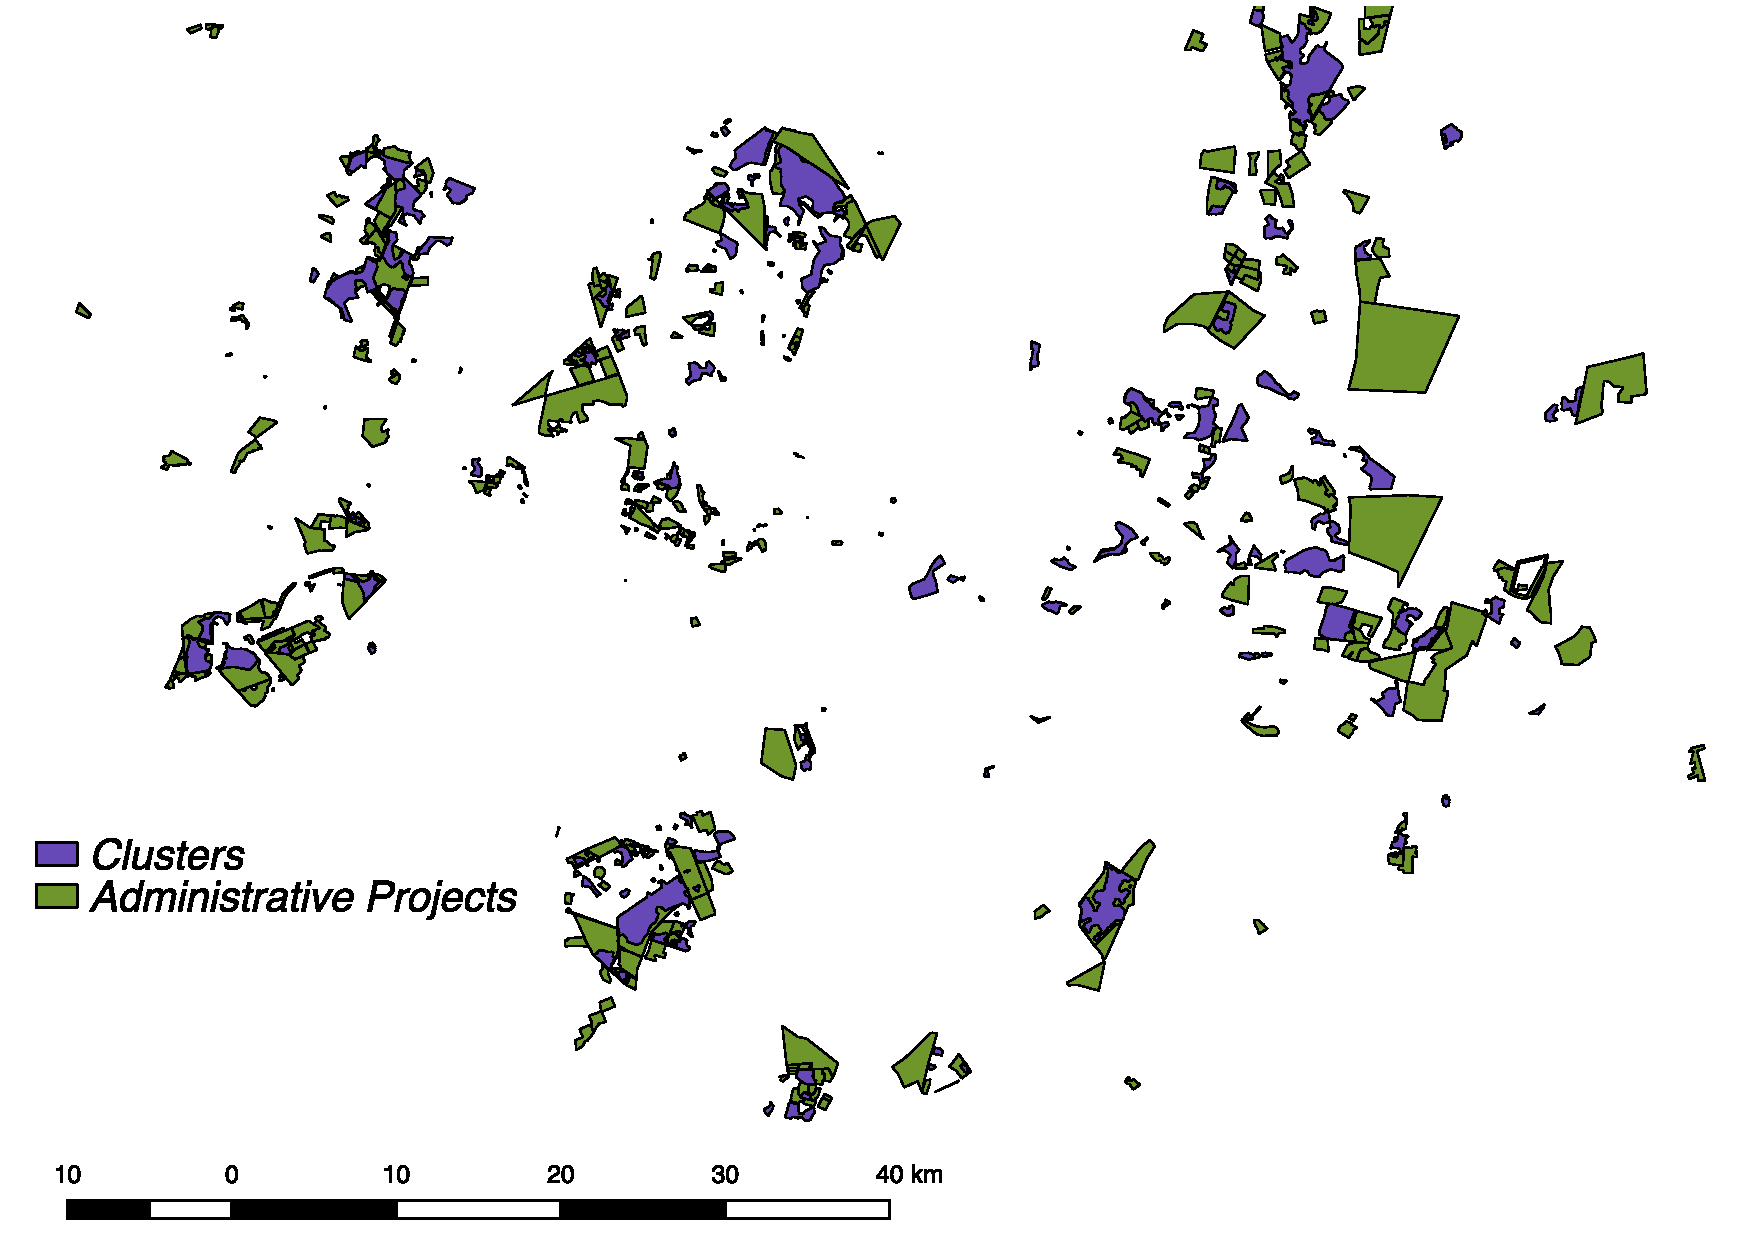
\includegraphics[scale=.5]{figures/gcro_convexhull_overlap.pdf} \\
This figure includes the northern half of housing projects.
\end{figure}

Table~\ref{table:projectdescriptives} provides descriptive statistics for the final sample of 56 completed and 101 uncompleted projects.  At baseline in the 2001 building census, we find that completed and uncompleted project areas have similar formal building density although uncompleted projects have much higher densities of informal structures.  Consistent with this finding, slum areas may face greater challenges in organizing funding as well as infrastructure provision necessary to complete large housing projects.  After project follow-through, completed areas experience dramatic increases in formal building density between 2001 and 2011 compared to uncompleted projects.  Both areas also experience substantial and similar growth in their levels of informal settlement growth.  The median year of completion as well as distance to Central Business District match well between completed and uncompleted projects 

\begin{table}
	\centering
	\caption{Housing Project Descriptives}\label{table:projectdescriptives}
\begin{tabu}{lcc}
 & Completed & Uncompleted \\ 
 Formal Density: 2001  & 340.6  & 89.1  \\ 
 Formal Density: 2011  & 1,783.1  & 491.1  \\ 
 &  &  \\ 
 Informal Density: 2001  & 443.0  & 1,569.2  \\ 
 Informal Density: 2011  & 1,064.6  & 1,993.4  \\ 
 &  &  \\ 
 Median Year (est.)  & 2005  & 2007  \\ 
 Distance to CBD (km)  & 28.9  & 27.6  \\ 
 &  &  \\ 
 Total Projects   & 56  & 35  \\ 
\bottomrule
\end{tabu}
\\
Density measures number structures per $\text{km}^2$. \\  Central Business Districts (CBD) are measured with respect to Johannesburg and Tshwane.
\end{table}

\section{Descriptive Evidence for Spillover Areas}\label{section:descriptives}

Examining the spillover effects of housing projects requires focusing the analysis on areas just around these housing projects, which may also limit the extent to which results may generalize more broadly.  To identify the spillover effects of public housing projects, we focus on all outcomes within a 1.2 kilometer buffer around each cluster.  Figure~\ref{figure:bufferdesign} shows an example.  Areas where buffers overlap are excluded to ensure that the empirical exercise is able to recover the impacts due to the nearest housing project.  

\begin{figure}
\caption{Buffer Design Properties Example}\label{figure:bufferdesign}
\centering
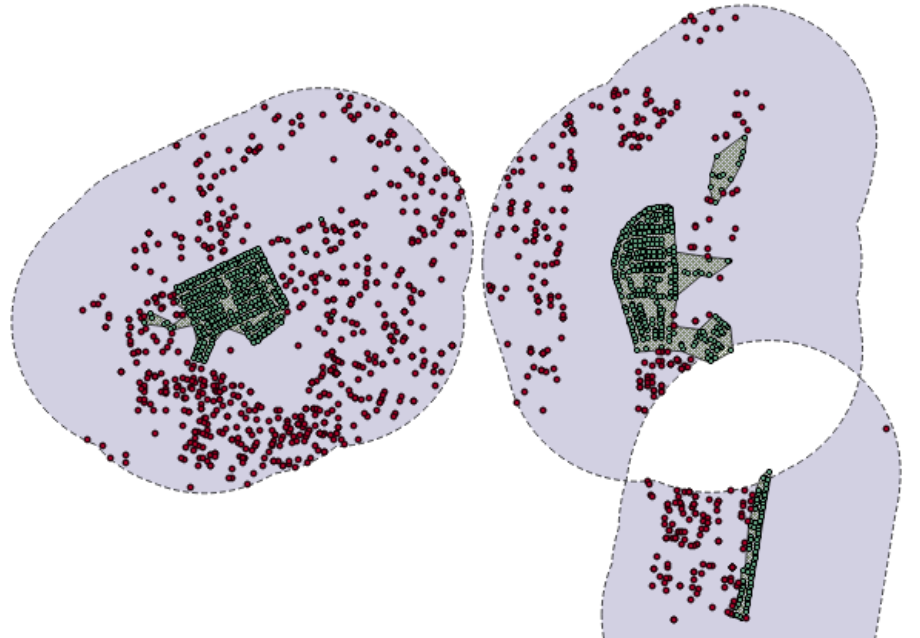
\includegraphics[scale=.4]{figures/design.png} 
\begin{itemize}
\item Project Properties : red circles
\item Non-Project Properties : dark green circles
\item Buffer Area (1.2 km from clusters) : light blue area
\end{itemize}
\end{figure}

To assess the extent to which these project areas are representative, Table~\ref{table:pricedescriptives} shows average characteristics for transactions in buffer areas for completed projects, buffer areas for uncompleted projects, and all other transactions outside of all buffer areas.  Average prices for completed projects closely resemble prices outside of buffer areas while uncompleted projects have much lower prices, supporting earlier evidence that these uncompleted projects are located in places with greater slum density.  Plot sizes for properties in completed and uncompleted project buffers are similar and much smaller than plots outside of these areas.  This finding is consistent with housing projects being located nearby dense residential or slum areas instead of in rural locations throughout the province.  Close to a third of all properties are sold multiple times and all share the same median purchase year.

\begin{table}
\caption{Property Prices within Buffer Areas}\label{table:pricedescriptives}
\centering
\begin{tabu}{lccc}
\toprule
 & Outside Buffer & Inside Buffer & Housing Project \\
\midrule
 Purchase Price (Rand)  & 184,199.6  & 205,891.3  & 142,748.8  \\ 
\rowfont{\footnotesize} & [386,165.1]  & [249,590.1]  & [447,771.6]  \\ 
 &  &  &  \\ 
 Plot Size (m3)  & 585.2  & 421.7  & 270.4  \\ 
\rowfont{\footnotesize} & [2,040.3]  & [1,225.7]  & [179.2]  \\ 
 &  &  &  \\ 
 Sold At Least Once  & 0.316  & 0.318  & 0.338  \\ 
 Median Purchase Year  & 2006  & 2006  & 2006  \\ 
 Distance to Project (meters) &  & 373.0  & \\
 \rowfont{\footnotesize} &  & [415.9]  & \\
\midrule
 Observations  & 275,296  & 94,172  & 108,809  \\ 
\bottomrule
\end{tabu}
 \\
Standard errors are in parentheses.  \\ This figure excludes transactions within project areas.
\end{table}

We use a similar buffer approach to examine census characteristics by including census blocks whose centroids fall within 1.2 km buffers of nearby projects.  Figure~\ref{figure:bufferdesigncensus} provides an example project that distinguishes between census blocks (in yellow) with greater than 30\% overlapping area with project areas and census blocks (in blue) with less than 30\% area overlap but whose centroids fall within the 1.2 km buffer.  This criteria allows for separating the direct effects of the housing projects within their footprint from the spillover effects of housing projects on the surrounding areas.  We focus on the 30\% area overlap threshold to account for cases where housing project areas are small relative to the nearest census blocks.

\begin{figure}
\caption{Buffer Design Census Block Example}\label{figure:bufferdesigncensus}
\centering
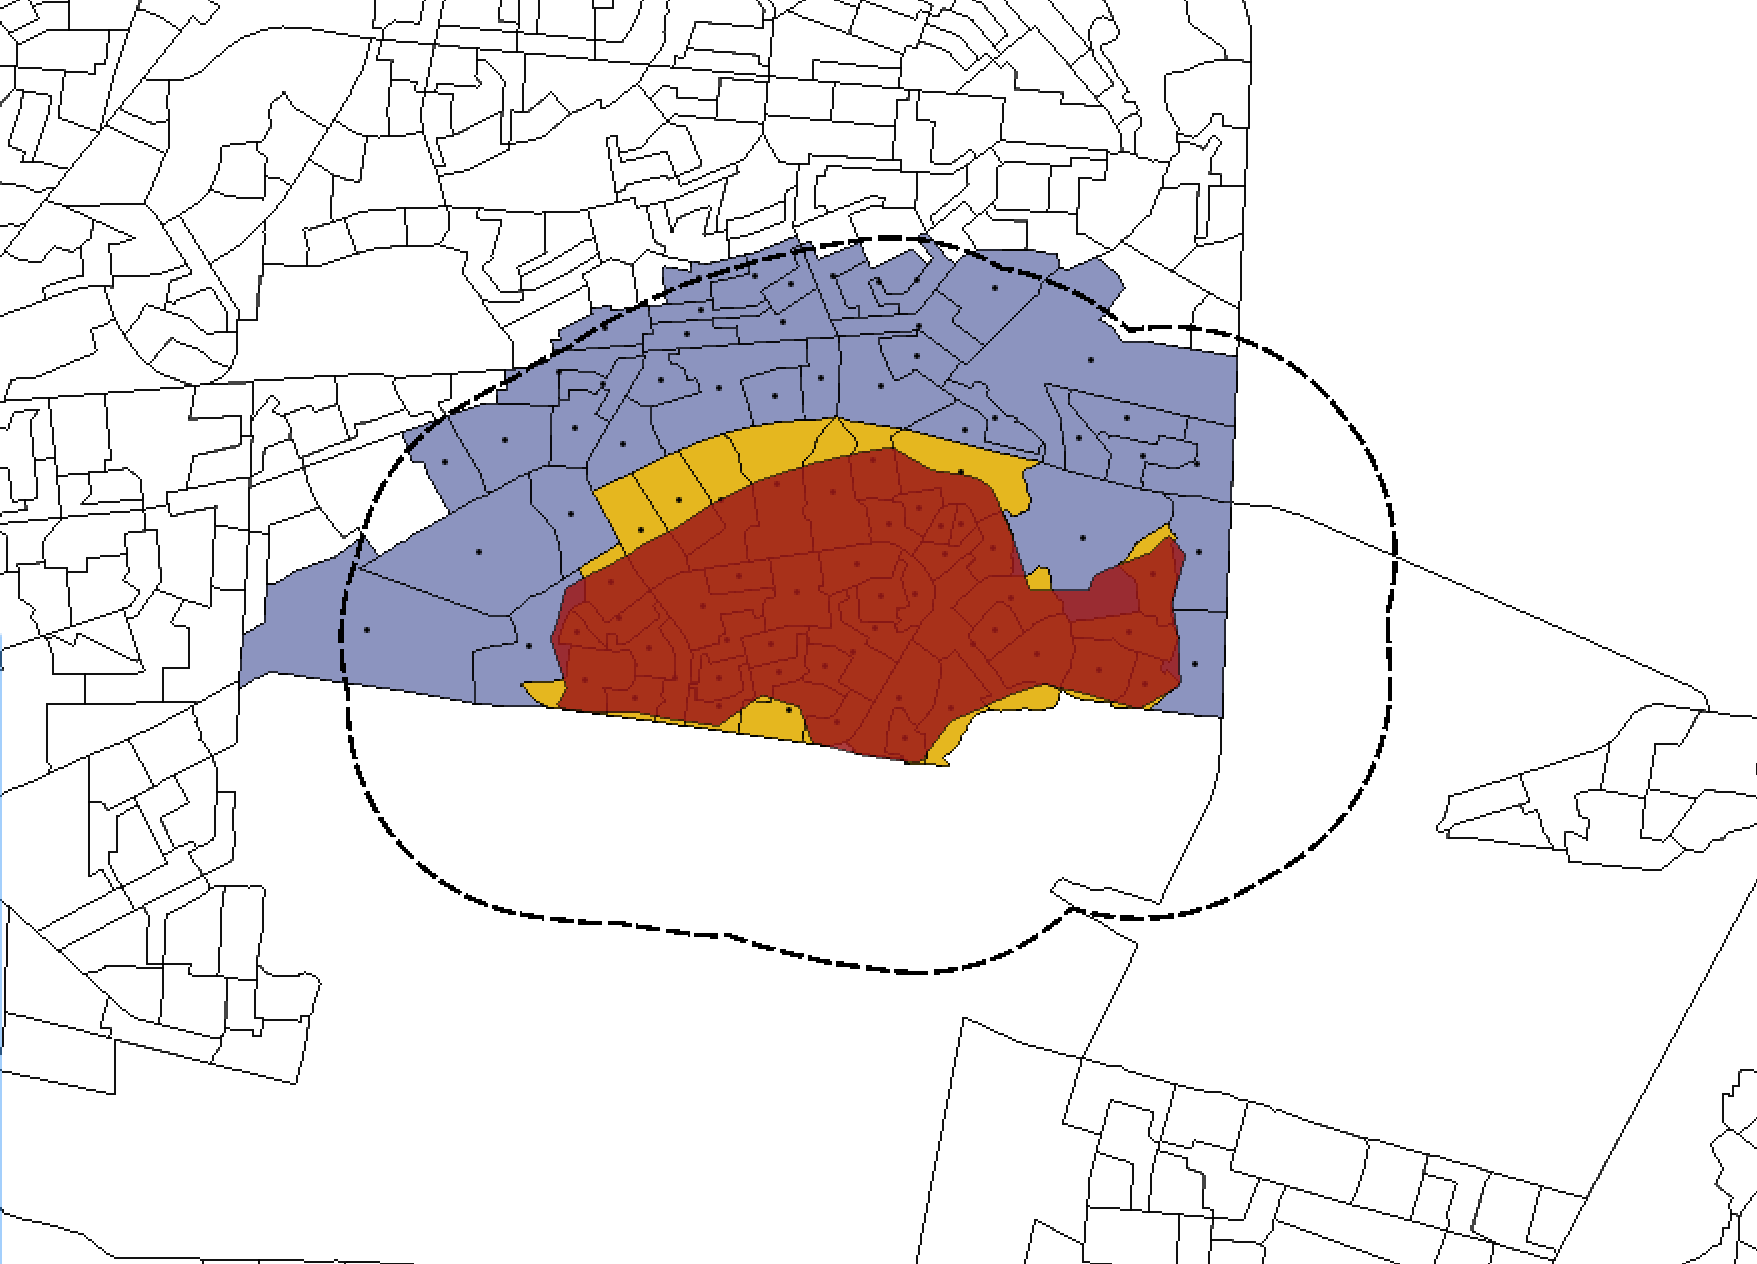
\includegraphics[scale=.4]{figures/design_7.png} 
\begin{itemize}
\item Census Blocks with $\geq$30\% project area overlap : yellow polygons 
\item Census Blocks with $<$30\% project area overlap : blue polygons
\item Buffer Area (1.2 km from clusters) : dotted line
\item Project Area : red polygon
\end{itemize}
\end{figure}

To compare census characteristics at baseline, Table~\ref{table:censusdescriptives} provides averages for households within and nearby both completed and uncompleted projects.  The first two columns find that relative to uncompleted project areas, census blocks within completed projects have much better infrastructure (flush toilets, piped water, and electricity), but have similar household sizes and are likely to own and reside in formal single houses.  Lower service provision in these areas matches previous evidence that uncompleted projects are often located near dense informal settlements.  These differences between uncompleted and completed projects disappear for census areas located just outside of project areas as shown in the last two columns.  Taken together, these results suggest that despite differences in service provision within project footprints at baseline, spillover areas may serve as useful comparison groups for each other.

\begin{table}
\caption{Census Characteristics in 2001 \\ by Overlap with Project Areas}\label{table:censusdescriptives}
\centering
\begin{tabu}{lcccc}
 & \multicolumn{2}{c}{Within Project}     & \multicolumn{2}{c}{Outside Project}    \\
 & \multicolumn{2}{c}{($>$30\% Overlap)}  & \multicolumn{2}{c}{($<$30\% Overlap)}   \\
 &  &  &  &  \\ 
 & Completed & Uncompleted & Completed  & Uncompleted  \\
\midrule
 Flush Toilet  & 0.56  & 0.18  & 0.77  & 0.82  \\ 
 &  &  &  &  \\ 
 Piped Water  & 0.21  & 0.07  & 0.41  & 0.36  \\ 
 &  &  &  &  \\ 
 Elec. Cooking  & 0.58  & 0.17  & 0.68  & 0.68  \\ 
 &  &  &  &  \\ 
 Elec. Light  & 0.79  & 0.23  & 0.74  & 0.82  \\ 
 &  &  &  &  \\ 
 Single House  & 0.51  & 0.45  & 0.52  & 0.59  \\ 
 &  &  &  &  \\ 
\midrule
 Observations  & 59,460  & 37,136  & 213,061  & 194,622  \\ 
\bottomrule
\end{tabu}
 \\
All variables are dummies for having each household attribute.
\end{table}

\subsection{Building Growth around Housing Projects}

Using the building structures survey, we provide a first look at housing development around completed and uncompleted projects.  Figure~\ref{figure:buildingchanges} plots the average number of new structures between 2001 and 2011 in distance rings from the boundary of both completed and uncompleted project areas.  Negative distances measure new structures within the project areas themselves.  

Focusing on completed projects in the left panel, strong growth in formal residential structures at negative distances provides another measure of the direct impact of the housing projects.  We also observe strong growth in informal residential structures within project areas.  This finding is consistent with anecdotal evidence from fieldwork in South Africa pointing to the prevalence of backyard shacks where owners of project houses use their land plots to construct informal housing.  At positive distances, the growth in formal structures immediately dissipates while the growth in informal structures remains substantial up to at least 400 meters from the project border.  This sustained growth in nearby informal dwellings matches a common complaint of local housing authorities and NGOs who notice crowding-in of slum areas around project areas in order to utilize the public services offered within the projects.  	

Results for uncompleted projects in the right panel indicate a similar pattern of informal structure growth in project areas.  However compared to completed projects, lower levels of formal structure growth occur within uncompleted project footprints before quickly dissipating outside of the projects.  Informal structure growth also decreases suddenly outside of the projects.  This result suggests that completed housing projects may play an important role in generating nearby growth in informal settlements in the right panel.  The flat, smooth trends in structure growth past 500 meters for both completed and uncompleted projects support interpreting these regions as capturing the types of local development that we might expect in the absence of the housing projects.

\begin{figure}
\caption{Growth in Structures between 2001 and 2011}\label{figure:buildingchanges}
\centering
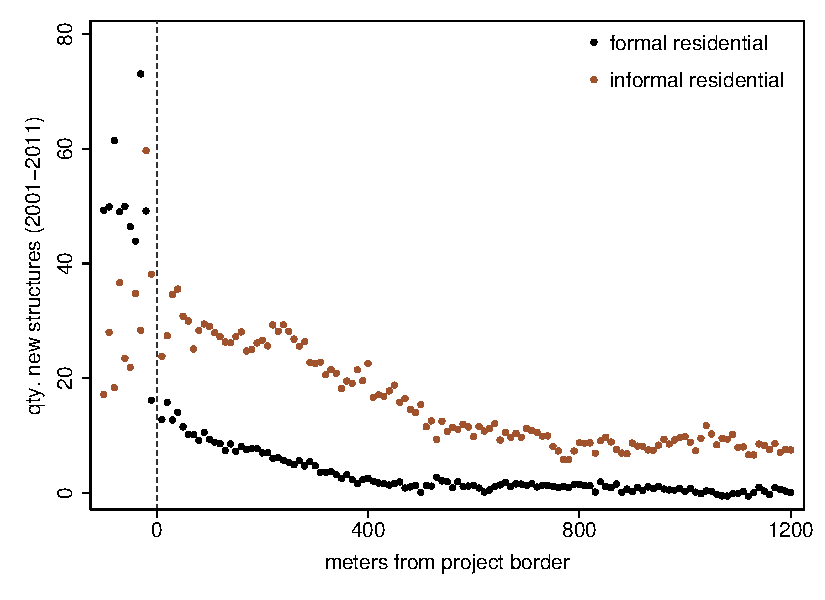
\includegraphics[scale=.58]{figures/bbluplot.pdf}
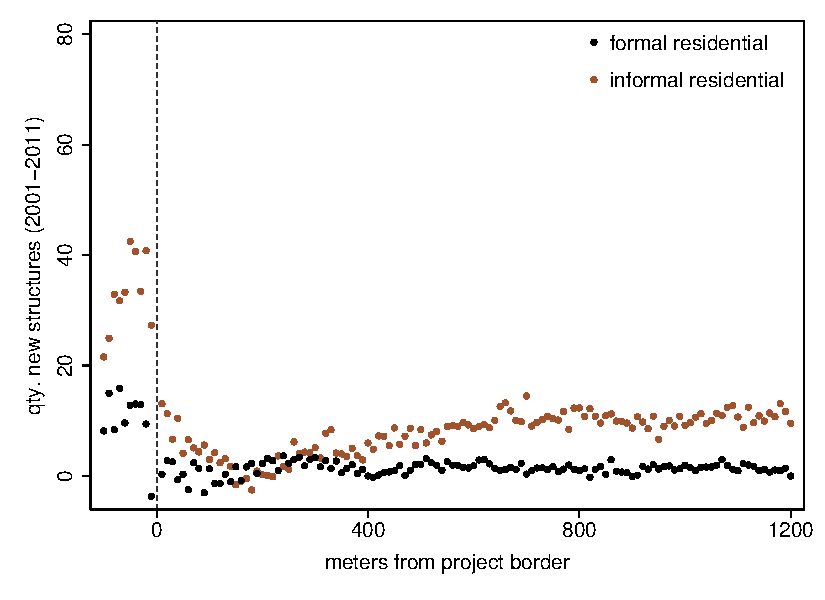
\includegraphics[scale=.58]{figures/bbluplot_placebo.pdf}\\
\hspace{.7cm} Completed Projects \hspace{4.2cm} Uncompleted Projects
\end{figure}



%\subsubsection{Pre-Existing Formal Dwellings:}  

% pre-existing transactions : 38468 / 127600 = 30\%

%We exclude transactions that occur on land plots with at least one preexisting formal residential structure in the 2001 building census (31\% of remaining transactions).  This method not only helps to reduce error in matching seller identities to housing programs, but also works to distinguish new housing projects from titling, home loan, or other programs that may have been implemented by local housing agencies over the same time period.   

%\subsubsection{Spatial Clustering:}  Since housing projects are characterized by large plots of adjacent dwellings, we use a density-based clustering algorithm to group transactions that satisfy the above criteria according to their geographic proximity.  By eliminating loosely clustered or singleton transactions, this method additionally helps to distinguish large housing projects from other small-scale housing programs.  

%Figure~\ref{figure:conhull} provides example convex hulls formed around project housing transactions.  The algorithm groups nearby transactions into two large projects on the right.  Some non-project transactions (pink circles) are also included in the convex hulls, which are likely miscoded project houses or privately constructed houses within housing projects.  The upper left collection of non-project houses contains a small group of houses coded as project houses (green circles).  However, since there are very few of these houses and they are loosely clustered within a large group of non-project houses, they are not identified as a convex hull.  These more isolated cases are likely to be small-scale land-titling programs or home-financing programs launching by local NGOs in collaboration with housing authorities.  

%\begin{figure}
%\caption{Convex Hull Example}\label{figure:conhull}
%\centering
%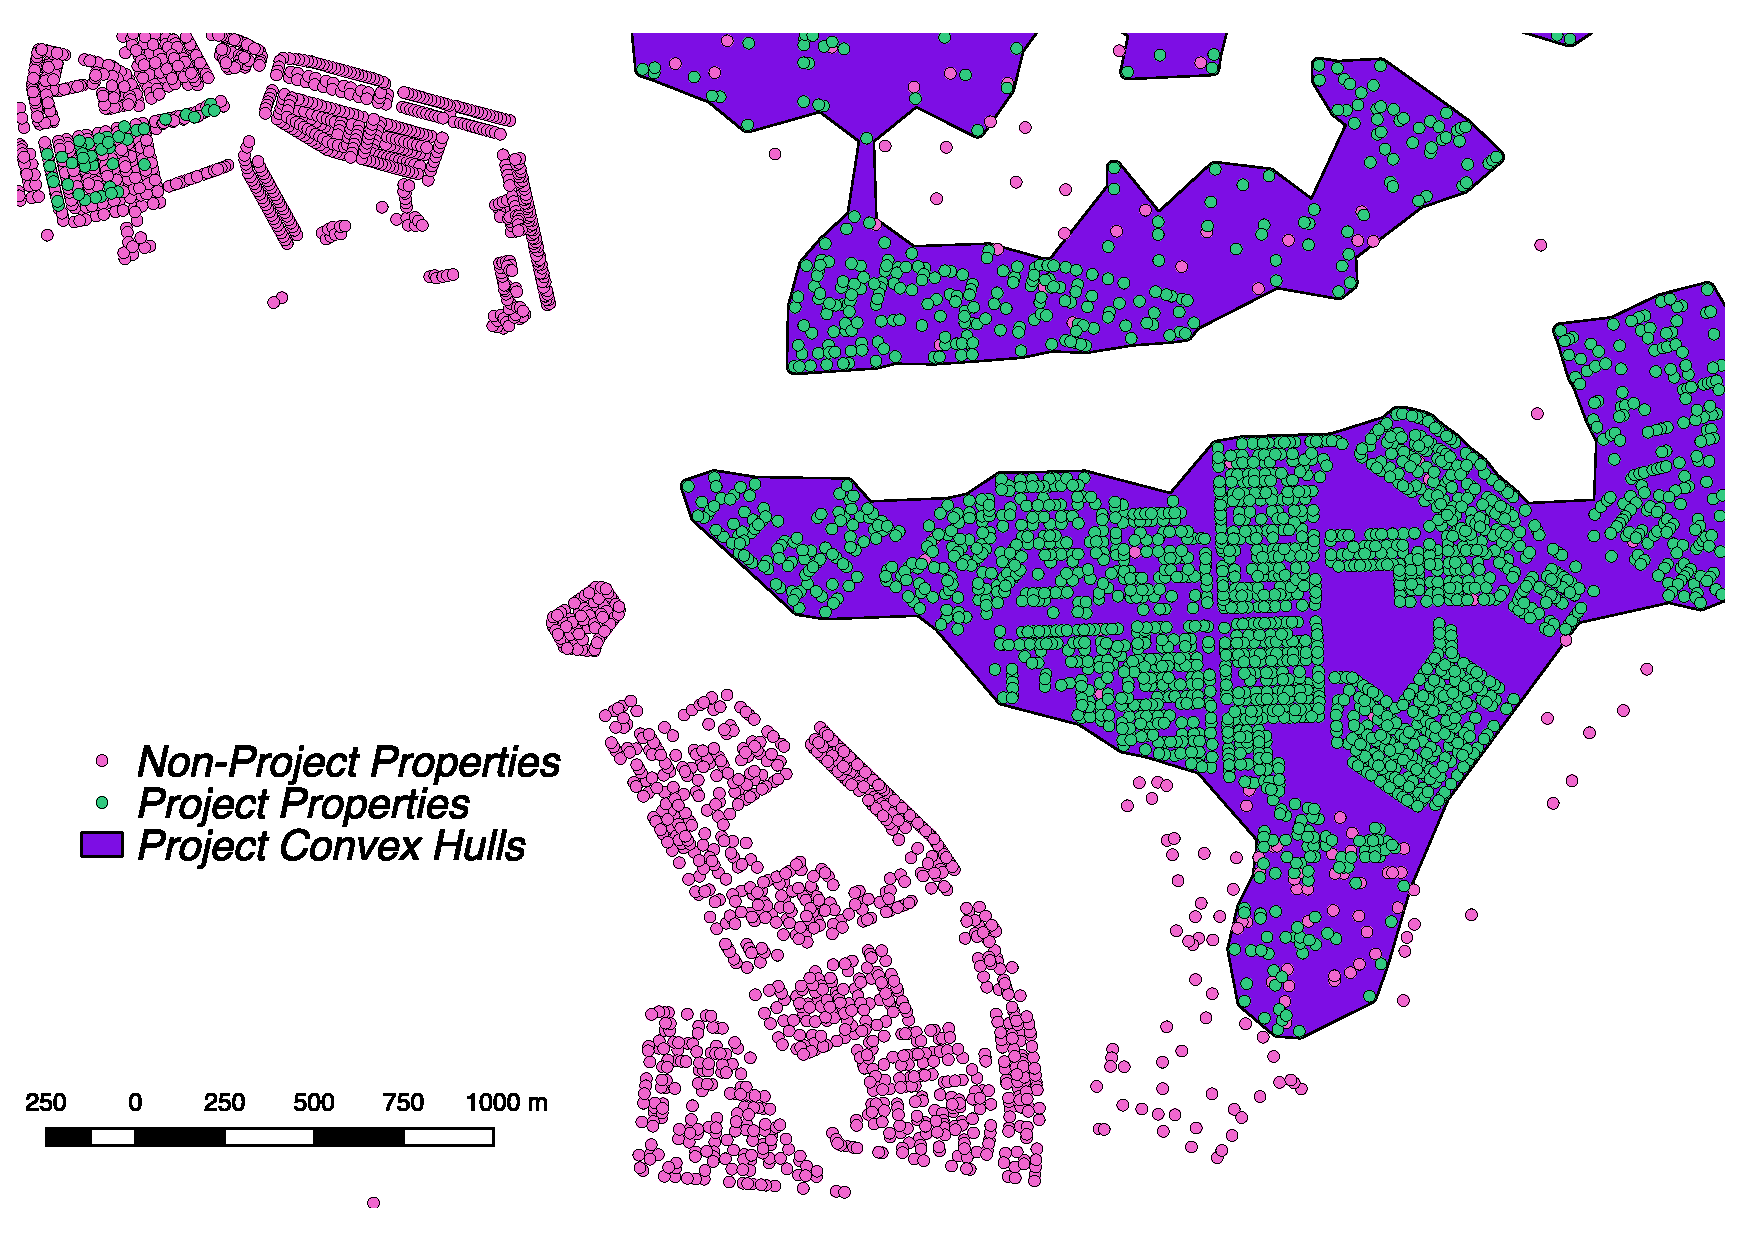
\includegraphics[scale=.5]{figures/convex_hull_v3_test.pdf}
%\end{figure}



\section{Results: Price Spillovers}\label{section:resultsprices}

To identify the spillover effects of public housing on residential home prices in the formal market, we use a difference-in-differences approach comparing prices for areas close and far from project areas before and after project implementation.  Our main empirical strategy takes the following specification:
\begin{equation*}
P_{itp} \, = \, \alpha D_{tp}T_{ip} \, + \,\theta_1 D_{tp} \, + \, \,\theta_2 T_{ip}+ \, X^{'}_{i}\beta \, +  \lambda_p \,  + \, \eta_{t} \, + \, \varepsilon_{itp}
\end{equation*}
The outcome, $P_{itp}$, is measured in terms of the log-purchase price of property $i$ sold at time $t$ in the vicinity of project $p$.  To capture changes in prices over time within project areas, $D_{tp}$ is equal to one if date $t$ is after the month of project implementation and zero otherwise.  $T_{ip}$ takes a value of one if property $i$ is within 400m of the project boundary (zero otherwise).  The coefficient of interest, $\alpha$ captures the differential change in prices between near and far properties before and after project construction.  $X_i$ controls for a quadratic in lot size, which can affect prices over time.  Additionally, $\lambda_p$ includes a project fixed affect controlling for any fixed, unobserved drivers of house prices that vary between projects.  Likewise, $\eta_{t}$ controls for calendar month (year$\,\times\,$month) fixed-effects to account for any factors such as shifts in aggregate housing demand that may be correlated with prices and the timing of housing projects.

Interpreting the coefficient, $\alpha$, as the causal effect of housing projects on nearby home prices requires the following assumption:
\begin{equation*}
E[\varepsilon_{itp}|X_{i},T_{ip},D_{tp},\lambda_p,\eta_{t}]=0
\end{equation*}
This assumption implies that there are no other factors occurring in the same time and place as the housing projects which may otherwise impact home prices.  One possibility is that housing markets anticipate the construction of these projects so that transactions in the pre-period may be partially treated by the advent of a housing project.  Anecdotal evidence suggests that completion dates for these projects are very uncertain due to the large coordination of stakeholders needed for each project, making it difficult to accurately anticipate implementation.  Another concern would be that housing projects are accompanied by other social programs that would stimulate investments in neighborhoods near project areas.  In order to isolate market anticipation or accompanying social programs from the actual impacts of housing projects, we estimate an identical model for planned but uncompleted projects to test the robustness of the results.

Similarly, in targeting housing projects to particular areas, governments may be responding to local trends in housing markets or economic conditions.  To separate project impacts from secular market trends, we leverage the sudden roll-out of housing projects under the assumption that market trends are relatively smooth over space and time relative to the construction of housing projects.  In order to non-parametrically assess identification in this way, we also estimate a more flexible model both in terms of distance to project, $D_{tp}$ and time relative to project construction, $T_{ip}$.  Specifically, we estimate separate treatment effects for each 100 meters of distance, $\sum_{d=100}^{1200} \alpha_d D_{tpd} T_{ip}$.  We also allow effects to vary according to two-month intervals relative to construction, $\sum_{l=-36}^{36} \alpha_l D_{tp}T_{ipl}$.  All regressions cluster standard errors at the project level in order to account for potentially correlation in prices due to unobserved factors within very localized housing markets.

Figure~\ref{figure:distplot} separately plots coefficients for average home prices before construction, $\alpha_{d,pre}$ and after construction, $\alpha_{d,post}$ for each 100m distance ring from housing project boundaries.  The left panel presents price gradients for completed projects.  The pre-project gradient slopes slightly upwards consistent with housing projects being located in undeveloped land or preexisting informal settlements.  After implementation, the price gradient slopes downwards sharply within 400 meters of the project area while remaining unchanged past this 400 meters threshold.  This result is consistent both with the growth of informal settlements concentrated in the same spatial interval as observed in Figure~\ref{figure:buildingchanges}.

Uncompleted projects in the right panel exhibit a flat price gradient before project implementation.  One explanation may be that since uncompleted projects are more often located in large slum neighborhoods, spillover areas may closely resemble these project areas.  After the estimated date of project completion, the price gradient remains flat shifting slightly, but noisily downward at all distances from the project boundary.  These findings suggest little local spillovers from the uncompleted projects alongside a deterioration in the local housing market affecting all properties evenly.  Additionally, these results provide suggestive evidence that exact location of housing projects does not appear to be strongly correlated with housing market trends at a very local level.

\begin{figure}
\caption{Price Estimates over Distance}\label{figure:distplot}
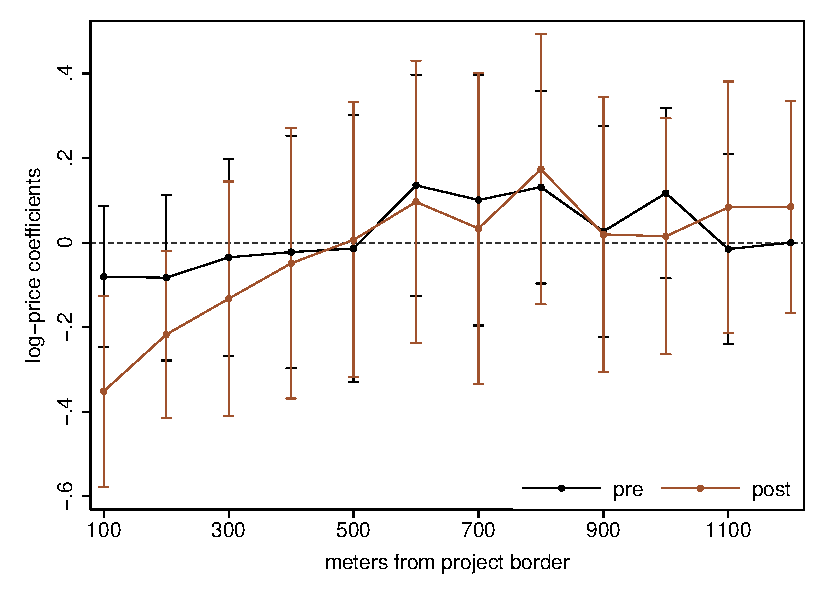
\includegraphics[width=0.5\textwidth,trim={.77cm 0cm .21cm 0cm}]{figures/distplot.pdf}
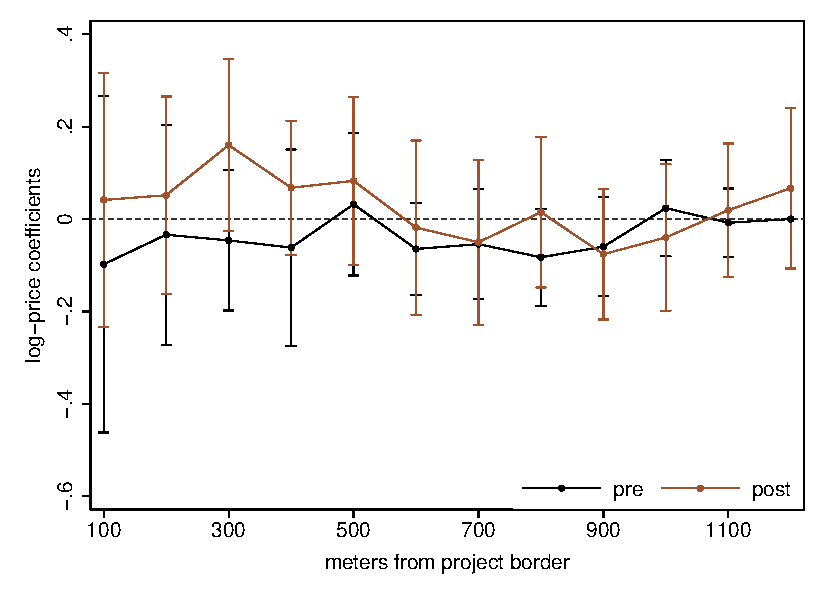
\includegraphics[width=0.5\textwidth,trim={.77cm 0cm .21cm 0cm},clip]{figures/distplot_placebo.pdf}\\
{\color{white}dddddddddddddd}Completed Projects \hspace{4.2cm} Uncompleted Projects
\end{figure}

Complementing these distance gradients, Figure~\ref{figure:timeplot} plots coefficients for average price changes over time relative to the modal construction month for properties within and beyond 400 meters of a project boundary.  Focusing on completed projects in the left panel, both areas far and near project boundaries follow a smooth, parallel evolution in prices over time.  This parallel trend provides evidence against large shifts in policy or economic conditions that may be correlated with the onset of these housing programs.  The price trajectories begin to deviate in the few months preceding the modal transaction date of the housing project.  While further away properties maintain a steady price level following the housing project, nearby properties experience a sustained dip in prices that persists up to three years after the project is implemented.  The sustained reduction in housing prices provides evidence for a lasting structural change in local housing market instead of a temporary resorting of households from nearby residences to project houses.  

The dip in prices begins in the couple months before the modal transaction year, which is consistent with nearby housing markets anticipating projects during their construction periods.  One hypothesis is that given the large observed decline in house prices, it would rational for housing markets to anticipate construction, producing a declining pretrend in prices before completion date.  The absence of an extended pretrend may speak to the unpredictability of the timing for these projects, especially given high coordination costs and frequent unplanned delays.

\begin{figure}
\caption{Price Estimates over Time}\label{figure:timeplot}
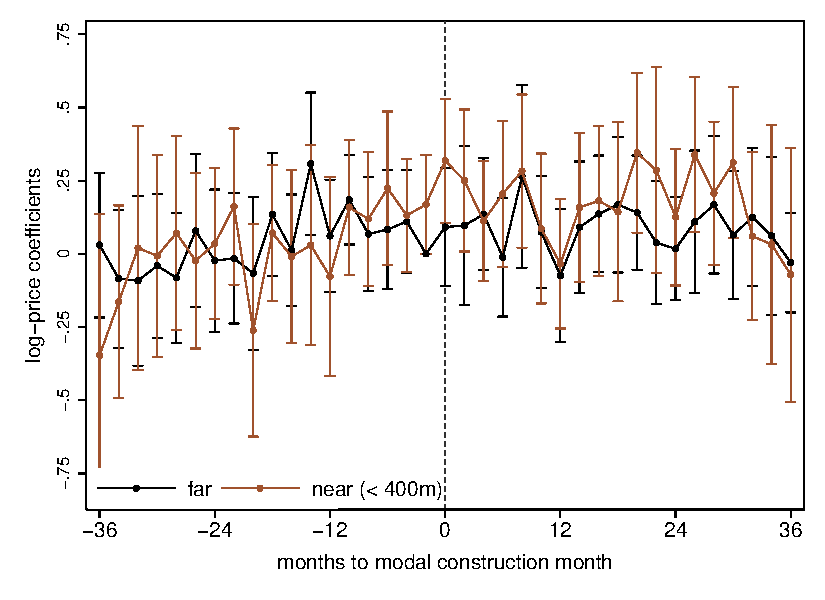
\includegraphics[width=0.5\textwidth,trim={.77cm 0cm .21cm 0cm}]{figures/timeplot.pdf}
   \hfill
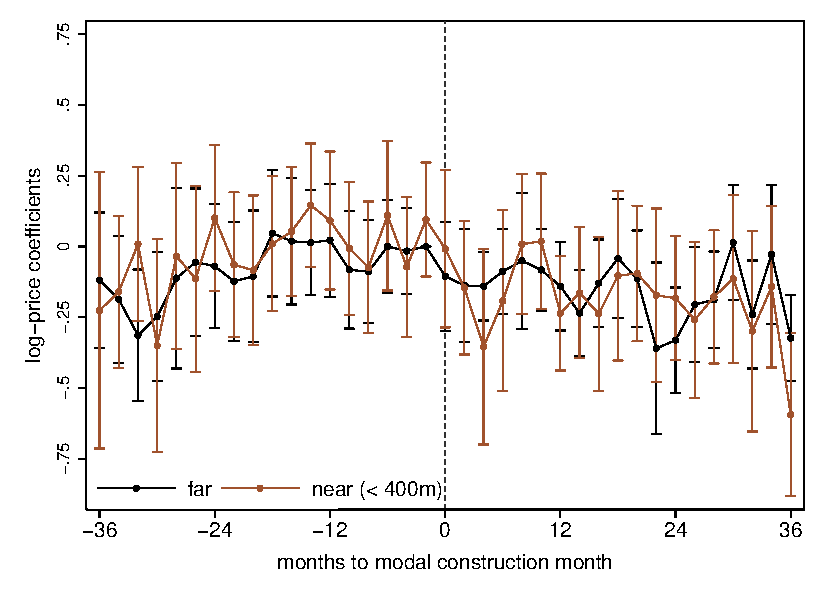
\includegraphics[width=0.5\textwidth,trim={.77cm 0cm .21cm 0cm},clip]{figures/timeplot_placebo.pdf}\\
{\color{white}dddddddddddddd}Completed Projects \hspace{4.2cm} Uncompleted Projects
\end{figure}

For uncompleted projects in the right panel, areas far and near project boundaries follow similar parallel trends to completed projects leading up to the expected completion date, but then remain indistinguishable for the entire duration after this date.  This null result helps to exclude competing explanations that rely on the timing of housing projects such as targeting housing programs according to hyper-local housing market trends or pairing housing projects with other place-based policies.  

Table~\ref{table:priceestcomplete} and Table~\ref{table:priceestplacebo} provide the difference-in-differences regression analogues to Figure~\ref{figure:distplot} and Figure~\ref{figure:timeplot}.  In the first column of Table~\ref{table:priceestcomplete}, we estimate a simple difference-in-differences specification and report the coefficient for properties within 400 meters of the project and 3 years of the start date.  Since the outcome is measured in log-prices, the coefficient indicates that housing prices in this range decline by 23.8\% as a result of the housing program.  Including project fixed-effects in the second column attenuates this effect to 16.6\% and reduces its statistical significance from 5\% to 10\% by accounting for fixed differences in the housing markets between clusters.  The third column disaggregates the coefficients by years following project completion.  Comparing coefficients, we only find a statistically significant coefficient for the first year of the project although effect sizes remain similar for all time intervals.  With just over 150 projects, significant noise in the housing price data, and a rich set of fixed effects, these specifications have difficulty precisely recovering price estimates.  In the spirit of Figure~\ref{figure:distplot}, the fourth column examines price effects at a finer spatial scale, finding an especially large and statistically significant price decline in the immediate 200 meters of a housing project which sharply attenuates past 200 meters.

\begin{table}
\caption{Price Estimates for Completed Projects}\label{table:priceestcomplete}
\centering
\begin{tabular}{lcccc} \hline
 & (1) & (2) & (3) & (4) \\
VARIABLES & Log Price & Log Price & Log Price & Log Price \\ \hline
 &  &  &  &  \\
3 yrs 0-400m & -0.238** & -0.166* &  &  \\
 & (0.106) & (0.0835) &  &  \\
1st yr 0-400m &  &  & -0.147* &  \\
 &  &  & (0.0754) &  \\
2nd yr 0-400m &  &  & -0.180 &  \\
 &  &  & (0.115) &  \\
3rd yr 0-400m &  &  & -0.118 &  \\
 &  &  & (0.0971) &  \\
3 yrs 0-200m &  &  &  & -0.224** \\
 &  &  &  & (0.0961) \\
3 yrs 200-400m &  &  &  & -0.0701 \\
 &  &  &  & (0.0664) \\
 &  &  &  &  \\
Observations & 28,701 & 28,701 & 28,701 & 28,701 \\
R-squared & 0.229 & 0.488 & 0.489 & 0.489 \\
Project FE & NO & YES & YES & YES \\
 Year-Month FE & YES & YES & YES & YES \\ \hline
\multicolumn{5}{c}{ Robust standard errors in parentheses} \\
\multicolumn{5}{c}{ *** p$<$0.01, ** p$<$0.05, * p$<$0.1} \\
\multicolumn{5}{c}{ All control for cubic in plot size. Standard errors are clustered at the project level.} \\
\end{tabular}

\end{table}

Table~\ref{table:priceestplacebo} repeats the same differences-in-differences exercise in Table~\ref{table:priceestcomplete} but for uncompleted projects.  Across all four columns, estimates are statistically insignificant and very small in magnitude compared to results in Table~\ref{table:priceestcomplete}.  In column three, we find one statistically significant coefficient at the 10\% level for price effects in third year, which appears to be driven by an outlier in the 36th month (according to the right panel in Figure~\ref{figure:timeplot}).  Taken together, these results provide additional evidence that price effects are primarily driven by the completion of housing projects rather than local trends in housing markets or economic conditions which would also affect uncompleted projects in theory.

\begin{table}
\caption{Price Estimates for Uncompleted Projects}\label{table:priceestplacebo}
\centering
\begin{tabular}{lcccc} \hline
 & (1) & (2) & (3) & (4) \\
VARIABLES & Log Price & Log Price & Log Price & Log Price \\ \hline
 &  &  &  &  \\
3 yrs 0-400m & -0.0435 & -0.0664 &  &  \\
 & (0.0784) & (0.0597) &  &  \\
1st yr 0-400m &  &  & -0.0687 &  \\
 &  &  & (0.0662) &  \\
2nd yr 0-400m &  &  & 0.00256 &  \\
 &  &  & (0.0729) &  \\
3rd yr 0-400m &  &  & -0.159* &  \\
 &  &  & (0.0841) &  \\
3 yrs 0-200m &  &  &  & -0.0365 \\
 &  &  &  & (0.0739) \\
3 yrs 200-400m &  &  &  & -0.0896 \\
 &  &  &  & (0.0624) \\
 &  &  &  &  \\
Observations & 24,562 & 24,562 & 24,562 & 24,562 \\
R-squared & 0.307 & 0.502 & 0.502 & 0.502 \\
Project FE & NO & YES & YES & YES \\
 Year-Month FE & YES & YES & YES & YES \\ \hline
\multicolumn{5}{c}{ Robust standard errors in parentheses} \\
\multicolumn{5}{c}{ *** p$<$0.01, ** p$<$0.05, * p$<$0.1} \\
\multicolumn{5}{c}{ All control for cubic in plot size. Standard errors are clustered at the project level.} \\
\end{tabular}

\end{table}


\section{Results: Infrastructure and Demographic Changes}\label{section:resultscensus}

To provide additional evidence on how the demographics and infrastructure may be changing as a result of these projects, we use slightly modified differences-in-differences design where uncompleted project areas are directly treated as counterfactuals.  The specification for analyzing the census data takes the following form:
\begin{equation*}
Y_{hbtp} \, = \, \alpha_{O} D_{tp} T_{bp} O_{bp} \, + \alpha_{S} D_{tp} T_{bp} S_{bp} \, + \,\theta_1 D_{tp} O_{bp} + \,\theta_2 D_{tp} S_{bp} \, + \theta_3 T_{bp} S_{bp}  \, +  \, \theta_4 S_{bp} \, +  \lambda_p \, + \, \varepsilon_{hbtp}
\end{equation*}
The outcome, $Y_{btph}$, includes demographic characteristics for household (or person) $h$ living in census block $b$ and project area $p$ in year $t$.  $O_{bp}$ takes a value of one for census blocks with greater than 30\% area overlap with housing projects (zero otherwise) while $S_{bp}$ is the converse identifying ``spillover'' census bocks that have less than 30\% overlap but whose centroids are still within a 1.2 km buffer of the housing project boundaries.  To account for secular changes in outcomes between 2001 and 2011 affecting all census blocks, $D_{tp}$ is equal to one if year $t$ is equal to 2011 and zero otherwise.  $T_{ip}$ takes a value of one for census blocks near completed projects and a value of zero for census blocks near uncompleted projects.  Controlling for differential time trends for overlap and spillover projects, $D_{tp} O_{bp} $ and $D_{tp} S_{bp}$ as well as separate means for both completed, $T_{bp} S_{bp}$, and uncompleted, $S_{bp}$, spillover areas leaves census blocks that overlap with uncompleted projects in the pre-period as the reference group.  $\lambda_p$ includes a project-level fixed effect to control for fixed differences in census characteristics between different projects.  The coefficients of interest, $\alpha_O$ and $\alpha_{S}$, capture differential changes in outcomes between completed and uncompleted projects separately for overlapping and spillover census blocks.  

To interpret the coefficients, $\alpha_O$ and $\alpha_S$, as the causal effects of housing projects on both overlapping and spillover outcomes, we make the following assumption:
\begin{equation*}
E[\varepsilon_{hitp}|T_{ip},D_{bp},S_{bp},O_{bp},\lambda_p]=0
\end{equation*}
Intuitively, this assumption requires that there are no other factors occurring at the same time both within and around the completed housing projects that may drive changes in local demographics.  By limiting the control group to only include uncompleted projects, we make the following parallel trends assumption: outcomes near completed projects would have evolved in the same ways as outcomes near uncompleted projects in the absence of the housing projects.  This design leverages similarities in areas around completed and uncompleted projects rather than comparing project areas to the entire region of Gauteng.  To the extent that locations of housing project may be targeted to local economic conditions, other areas in the province may be less likely to satisfy parallel trends assumptions.  

At the same time, local economic and political conditions may determine which projects are completed and which are either canceled or delayed.  To the extent that these conditions may be correlated with changes in local demographics, the assumption of parallel trends would not hold in the analysis.  Table~\ref{table:censusdescriptives} and Table~\ref{table:projectdescriptives} provide evidence that uncompleted project areas have more informal settlements and fewer services at baseline, consistent with policymakers placing less priority on finishing projects in these areas.  At the same time, spillover areas appear very similar in Table~\ref{table:censusdescriptives} suggesting that differences in trends in these areas may be more plausibly associated with completion of housing projects.  

Table~\ref{table:censusestimates} provides difference-in-differences estimates for a range of household level outcomes.  The first two rows include the coefficients of interest, which measure the differential change in outcomes for completed and uncompleted projects.  The first row reports effects for census blocks with greater than 30\% overlap (Project) and the second row includes census blocks with less than 30\% overlap (Spillover).  Broadly, infrastructure and home quality measures (flush toilet, piped water, single house, and number of rooms) increase in overlapping areas while these same measures decrease in spillover areas.  Many effects ares statistically significant at the 5 to 1\% level and are large in magnitude.  For example, the first column predicts a 21\% increase in piped water for project areas with a corresponding decrease of 7\% in spillover areas.  While we observe large changes in infrastructure provision, estimates are small and insignificant for household size and home ownership.

The third and fourth rows capture secular changes in outcomes over time for uncompleted project areas.  These measures indicate large overall increases in infrastructure and home quality measures in roughly similar magnitudes for spillover and project areas.

\begin{table}
\caption{Census Household-level Estimates}\label{table:censusestimates}
\centering
\begin{adjustbox}{angle=90}
\resizebox{\textheight}{!}{  
{
\def\sym#1{\ifmmode^{#1}\else\(^{#1}\)\fi}
\begin{tabular}{l*{5}{c}}
\hline\hline
          &\multicolumn{1}{c}{(1)}         &\multicolumn{1}{c}{(2)}         &\multicolumn{1}{c}{(3)}         &\multicolumn{1}{c}{(4)}         &\multicolumn{1}{c}{(5)}         \\
\hline
1.ptreat#1.gr&    0.269\sym{**} &    0.239\sym{***}&    0.027         &   -0.030         &    0.213\sym{***}\\
          &  (0.103)         &  (0.060)         &  (0.107)         &  (0.136)         &  (0.051)         \\
[1em]
1.ptreat#2.gr&   -0.031         &   -0.068\sym{**} &   -0.114\sym{***}&   -0.020         &   -0.069\sym{**} \\
          &  (0.037)         &  (0.034)         &  (0.042)         &  (0.033)         &  (0.033)         \\
\hline
\(N\)     &  1360081         &  1360081         &  1360081         &  1360081         &  1307418         \\
\(R^{2}\) &    0.353         &    0.213         &    0.250         &    0.241         &    0.156         \\
\hline\hline
\multicolumn{6}{l}{\footnotesize Standard errors in parentheses}\\
\multicolumn{6}{l}{\footnotesize \sym{*} \(p<0.10\), \sym{**} \(p<0.05\), \sym{***} \(p<0.01\)}\\
\end{tabular}
}

%Project census blocks have $>$30\% project overlap.  Spillover census blocks have $\leq$30\% project overlap.
}
\end{adjustbox}
\end{table}

Table~\ref{table:censusestimatesperson} repeats the same exercise focusing on changes in demographic composition for households living in these areas.  In the first row of column one, we find a statistically significant decrease in the share of high school (or greater) educated adults by around 3.6\%.  One explanation is that the housing policies are able to target recipients based on means and many of the original beneficiaries continue to reside in project areas.  For spillover areas and measures of household income and employment, we find no detectable effects of the housing program.

\begin{table} 
\caption{Census Person-level Demographic Estimates}\label{table:censusestimatesperson}
\centering 
\begin{tabular}{lccc} \hline
 & (1) & (2) & (3) \\
VARIABLES & Over HS Educ. & HH Income & Unemployed \\ \hline
 &  &  &  \\
Project X Post X Complete & -0.0360*** & -96.45 & 0.00604 \\
 & (0.0117) & (395.0) & (0.0222) \\
Spillover X Post X Complete & -0.00455 & 22.31 & 0.0200 \\
 & (0.0125) & (476.6) & (0.0159) \\
Project X Post & 0.0786*** & 705.2*** & -0.142*** \\
 & (0.00946) & (252.2) & (0.0110) \\
Spillover X Post & 0.0298*** & 2,231*** & -0.134*** \\
 & (0.00684) & (288.1) & (0.00801) \\
Spillover X Complete & -0.0194 & -1,425*** & 0.0299 \\
 & (0.0156) & (532.9) & (0.0220) \\
Spillover & 0.0236* & 860.2* & -0.0591*** \\
 & (0.0138) & (455.4) & (0.0159) \\
Constant & 0.825*** & 2,460*** & 0.505*** \\
 & (0.00600) & (244.7) & (0.00837) \\
 &  &  &  \\
Observations & 2,191,516 & 972,949 & 1,145,850 \\
R-squared & 0.028 & 0.062 & 0.057 \\
 Project FE & YES & YES & YES \\ \hline
\multicolumn{4}{c}{ Robust standard errors in parentheses} \\
\multicolumn{4}{c}{ *** p$<$0.01, ** p$<$0.05, * p$<$0.1} \\
\multicolumn{4}{c}{ Standard errors are clustered at the project level.} \\
\end{tabular}

\end{table}


\section{Discussion}\label{section:discussion}

Within the framework of US housing policy analysis in \cite{diamond2016wants}, South African housing projects would likely be considered as positive amenities at least within their footprints.  Housing projects successfully deliver large numbers of new structures (Figure~\ref{figure:buildingchanges}) and much better access to bulk services (Table~\ref{table:censusestimates}).  Results in Table~\ref{table:censusestimates} and Table~\ref{table:censusestimatesperson} also indicate that these new project houses are at least as good as neighboring houses at baseline while program beneficiaries share similar demographics to their neighbors.  Therefore, consistent with the model in \cite{diamond2016wants}, we would expect to find that these programs increase nearby home prices; however, models from developed contexts often do not take into account the presence of informal markets and associated congestion externalities.  

In the context of South Africa, we find evidence of complementarities between public housing programs and informal housing markets, which have large implications for prices in nearby formal housing markets.  Just outside of their footprints, housing projects lead to large increases in slums demonstrated both in terms of more informal structures in Figure~\ref{figure:buildingchanges} as well as greater shares of unserviced and informal housing from census data in Table~\ref{table:censusestimates}.  We hypothesize that informal housing markets benefit both from greater access to public services as well as newly zoned and cleared land around housing projects.  

Using both time and geographic variation in housing projects in Table~\ref{table:priceestcomplete}, we find that formal home prices decline substantially and overlap geographically with observed growth in slums.  The persistence of these declines in formal home prices supports the interpretation of these projects as representing structural shifts rather than temporary readjustments in local housing markets.  Given the high quality of the project houses themselves, we interpret this decline as more associated with the sudden increase in nearby informal settlements than due to any disamenities created by the project houses.  Taken together, these results suggest that complementarities between housing projects and slum growth may outweigh any amenity gains from the housing projects themselves and work to impede formal development in neighborhoods surrounding these projects.

\section{Conclusion}\label{section:conclusion}

This paper serves as a cautionary tale for low-density public housing in developing countries.  While these projects may be designed to improve local housing markets and reduce local slum growth, they may instead support local slum growth through a mix of available land and improved infrastructure.  It is important to emphasize that our analysis does not currently speak to the overall welfare implications of these policies.  For example, public housing may lead to an overall net reduction in slums in the city, which may generate total welfare gains through fewer congestion externalities or other mechanisms.  According to our model, the optimal housing policy depends crucially on the shape of these congestion externalities.  We look forward to using variation in the South African housing program to estimate these externalities in future work.  In light of South Africa's emphasis on using housing policy to stimulate neighborhood development, we hope that this paper will be useful for policymakers in considering the range of informal housing market responses as they design new housing policy.






{}
\nocite{*}
\singlespacing
\setlength\bibsep{0pt}
\bibliographystyle{abbrvnat}
\bibliography{ref}




% APPENDIX 
\appendix
\doublespacing

\section*{Appendix}

\begin{table}
	\centering
	\caption{Assessing Name Matching between \\Budget and Spatial Administrative Data}\label{table:stringmatch}
\begin{tabu}{lcc}
 & Matched  & Unmatched  \\
\midrule
 Formal Density: 2001  & 230.5  & 171.5  \\ 
 Formal Density: 2011  & 814.1  & 444.0  \\ 
 &  &  \\ 
 Informal Density: 2001  & 1,055.6  & 1,401.0  \\ 
 Informal Density: 2011  & 1,613.2  & 2,147.0  \\ 
 &  &  \\ 
 Project House Density  & 125.0  & 66.0  \\ 
 Project Mode Year  & 2005  & 2005  \\ 
 &  &  \\ 
 Hectares  & 97.3  & 119.6  \\ 
 &  &  \\ 
\midrule
 Observations  & 322  & 320  \\ 
\bottomrule
\end{tabu}
 \\
Density is measured in structures per $\text{km}^{2}$.

\end{table}


\end{document}